\chapter{Hierarchical Knowledge Architecture}

\begin{tcolorbox}[colback=blue!5!white,colframe=blue!75!black,title=Chapter Summary]
This chapter establishes the complete architectural framework of the Elder Heliosystem, bridging the mathematical foundations of Units I and II with the practical implementation of a hierarchical knowledge system. We begin by formalizing the connection between heliomorphic functions and the Elder-Mentor-Erudite architecture, showing how the abstract mathematical structures manifest in a concrete computational system. The chapter then presents the comprehensive hierarchical design that enables knowledge representation and transfer across multiple levels of abstraction, from universal principles in the Elder entity to domain-specific implementations in Erudite entities.
\end{tcolorbox}

\section{From Heliomorphic Functions to System Architecture: The Final Bridge from Unit II to Unit III}

Before detailing the complete Elder Heliosystem architecture, we must establish a rigorous mathematical mapping that shows how the heliomorphic function framework developed in Unit II manifests in the concrete computational structures of Unit III. This formal bridge between theoretical mathematics and implementation is essential for ensuring that the abstract principles of Elder Theory are preserved in the practical realization.

\begin{definition}[Elder Heliosystem Structure]
\label{def:heliosystem_structure}
The Elder Heliosystem $\mathcal{H}$ is defined as the computational implementation of the Elder Theory, consisting of:
\begin{equation}
\mathcal{H} = (\mathcal{E}, \{\mathcal{M}_i\}_{i=1}^D, \{\mathcal{E}r_{i,j}\}_{i=1,j=1}^{D,N_i}, \Omega, \Phi)
\end{equation}
where:
\begin{itemize}
    \item $\mathcal{E}$ is the Elder entity, capturing universal cross-domain principles
    \item $\{\mathcal{M}_i\}_{i=1}^D$ is the set of $D$ Mentor entities, each specializing in a domain
    \item $\{\mathcal{E}r_{i,j}\}_{i=1,j=1}^{D,N_i}$ are the Erudite entities, where $\mathcal{E}r_{i,j}$ is the $j$-th Erudite under the $i$-th Mentor
    \item $\Omega = \{\omega_E, \{\omega_{M_i}\}, \{\omega_{Er_{i,j}}\}\}$ is the set of orbital frequencies
    \item $\Phi = \{\phi_E, \{\phi_{M_i}\}, \{\phi_{Er_{i,j}}\}\}$ is the set of phase relationships
\end{itemize}
\end{definition}

\begin{theorem}[Canonical Isomorphism from Heliomorphic Functions to Heliosystem Architecture]
\label{thm:helio_to_architecture}
Given the isomorphism $\Psi: \elder{d} \rightarrow \mathcal{HL}(\mathcal{D})$ from Elder spaces to heliomorphic functions established in Theorem \ref{thm:elder_heliomorphic_isomorphism}, there exists a canonical implementation mapping $\mathcal{I}: \mathcal{HL}(\mathcal{D}) \rightarrow \mathcal{H}$ from heliomorphic functions to the Elder Heliosystem architecture such that the composition $\mathcal{I} \circ \Psi$ preserves all relevant mathematical structures from Unit I through Unit III.

The mapping $\mathcal{I}$ satisfies:
\begin{enumerate}
    \item \textbf{Hierarchical Level Correspondence:} Radial coordinates $r$ in heliomorphic functions map to hierarchical levels in the Elder-Mentor-Erudite system through:
    \begin{align}
        \mathcal{I}(f|_{r=r_E}) &= \Theta_E \quad \text{(Elder parameters)} \\
        \mathcal{I}(f|_{r=r_{M_i}}) &= \Theta_{M_i} \quad \text{(Mentor parameters for domain $i$)} \\
        \mathcal{I}(f|_{r=r_{Er_{i,j}}}) &= \Theta_{Er_{i,j}} \quad \text{(Erudite parameters for the $j$-th Erudite in domain $i$)}
    \end{align}
    where $r_E < r_{M_i} < r_{Er_{i,j}}$ for all $i,j$, reflecting the gravitational hierarchy.
    
    \item \textbf{Domain Specialization Correspondence:} Angular coordinates $\theta$ map to domain specializations through:
    \begin{equation}
        \mathcal{I}(f|_{\theta=\theta_i}) = \text{Parameters for domain $i$ across all hierarchical levels}
    \end{equation}
    
    \item \textbf{Magnitude-Parameter Correspondence:} The magnitude component $\rho(r,\theta)$ maps to parameter importance in the computational system:
    \begin{equation}
        |\Theta_{X,i}| = \rho(r_X, \theta_i)
    \end{equation}
    where $\Theta_{X,i}$ is the $i$-th parameter in entity $X$ (which can be Elder, Mentor, or Erudite).
    
    \item \textbf{Phase-Relation Correspondence:} The phase component $\phi(r,\theta)$ maps to relational properties that enable knowledge transfer:
    \begin{equation}
        \arg(\Theta_{X,i}) = \phi(r_X, \theta_i)
    \end{equation}
    
    \item \textbf{Gravitational Field Preservation:} The gravitational field structure from heliomorphic functions is preserved in the implementation through the gravitational field parameters of the heliosystem:
    \begin{equation}
        G_{\mathcal{H}}(r, \phi) = \gamma(r)e^{i\beta(r,\theta)}
    \end{equation}
    where $G_{\mathcal{H}}$ is the gravitational field function in the heliosystem, and $\gamma(r)$ and $\beta(r,\theta)$ are the gravitational field parameters from the heliomorphic differential equations.
\end{enumerate}
\end{theorem}

\begin{proof}
We construct the implementation mapping $\mathcal{I}$ explicitly. Given a heliomorphic function $f(re^{i\theta}) = \rho(r,\theta)e^{i\phi(r,\theta)}$, we define:

1. \textbf{Parameter Assignment:} For each entity in the heliosystem, we assign parameter values based on the heliomorphic function values at specific radii and angles:
\begin{align}
\Theta_E &= \{f(r_E e^{i\theta_k}) \mid k \in \text{indices for Elder parameters}\} \\
\Theta_{M_i} &= \{f(r_{M_i} e^{i\theta_k}) \mid k \in \text{indices for Mentor $i$ parameters}\} \\
\Theta_{Er_{i,j}} &= \{f(r_{Er_{i,j}} e^{i\theta_k}) \mid k \in \text{indices for Erudite $j$ under Mentor $i$ parameters}\}
\end{align}

2. \textbf{Orbital Dynamics:} The orbital frequencies and phases in the heliosystem are derived from the phase dynamics of the heliomorphic function:
\begin{align}
\omega_E &= \left.\frac{\partial \phi(r,\theta)}{\partial \theta}\right|_{r=r_E} \\
\omega_{M_i} &= \left.\frac{\partial \phi(r,\theta)}{\partial \theta}\right|_{r=r_{M_i}, \theta=\theta_i} \\
\omega_{Er_{i,j}} &= \left.\frac{\partial \phi(r,\theta)}{\partial \theta}\right|_{r=r_{Er_{i,j}}, \theta=\theta_{i,j}}
\end{align}

3. \textbf{Gravitational Field Implementation:} The gravitational field tensor $\mathcal{T}_f$ from the heliomorphic function is implemented in the computational system through the gravitational parameters of each entity and their interaction strengths.

The canonical property of this mapping follows from the construction, which preserves all the structural properties of the heliomorphic functions in the computational implementation. The preservation of Elder space structures follows from the composition with the isomorphism $\Psi$ established in Theorem \ref{thm:elder_heliomorphic_isomorphism}.
\end{proof}

\begin{theorem}[Implementation Completeness and Soundness]
\label{thm:implementation_completeness}
The mapping $\mathcal{I}: \mathcal{HL}(\mathcal{D}) \rightarrow \mathcal{H}$ from heliomorphic functions to the Elder Heliosystem is:

1. \textbf{Complete:} For any heliomorphic function $f \in \mathcal{HL}(\mathcal{D})$ within the relevant domain, there exists a parameter configuration in the Elder Heliosystem that implements it:
\begin{equation}
\forall f \in \mathcal{HL}(\mathcal{D}), \exists \boldsymbol{\Theta} = (\Theta_E, \{\Theta_{M_i}\}, \{\Theta_{Er_{i,j}}\}) \text{ such that } \mathcal{I}(f) = \boldsymbol{\Theta}
\end{equation}

2. \textbf{Sound:} Any valid configuration of the Elder Heliosystem corresponds to a well-defined heliomorphic function:
\begin{equation}
\forall \boldsymbol{\Theta} \in \Theta_E \times \prod_{i=1}^D \Theta_{M_i} \times \prod_{i=1}^D \prod_{j=1}^{N_i} \Theta_{Er_{i,j}}, \exists f \in \mathcal{HL}(\mathcal{D}) \text{ such that } \mathcal{I}(f) = \boldsymbol{\Theta}
\end{equation}
\end{theorem}

\begin{corollary}[Theoretical Property Preservation]
\label{cor:property_preservation}
All theoretical properties established for Elder spaces in Unit I and heliomorphic functions in Unit II are preserved in the computational implementation of the Elder Heliosystem in Unit III, including:

1. Phase coherence properties
2. Gravitational stratification
3. Hierarchical information flow
4. Transfer learning capabilities
5. Convergence guarantees for learning algorithms
\end{corollary}

This formal bridge establishes that the Elder Heliosystem is not merely inspired by the mathematical theory but is a direct implementation that preserves all essential properties. This ensures that the theoretical results from Units I and II—including knowledge transfer mechanisms, phase-coherence properties, and convergence guarantees—translate directly to the practical implementation in Unit III.

\section{Complete System Architecture}

Building on the mathematical foundation established in the preceding sections, we now present the complete architectural design of the Elder framework and the Elder-Mentor-Erudite hierarchy. This framework operates on structured data in the magefile format, which contains both spatial and temporal information derived from multiple sources. The hierarchical knowledge structure enables the system to learn at multiple levels of abstraction, from universal principles in the Elder Manifold to domain-specific knowledge in Erudites. This hierarchical knowledge organization facilitates systematic knowledge decomposition where abstract principles guide concrete implementations across domains.

\subsection{Learning Rate Stability Analysis}

The learning rate establishes a deterministic relationship that fundamentally governs the eventual stability or instability of the Elder system through precise mathematical mechanisms. This deterministic relationship between learning rate and system stability exhibits predictable patterns where lower learning rates result in slower learning but higher likelihood of convergence to stable solutions. The mathematical foundation of this deterministic relationship can be formalized as:

\begin{theorem}[Learning Rate Stability Relationship]
For the Elder-Mentor-Erudite system with learning rate $\eta$, the probability of system stability $P_{\text{stable}}(\eta)$ satisfies:
\begin{equation}
P_{\text{stable}}(\eta) = 1 - \exp\left(-\frac{\eta_{\text{critical}}}{\eta}\right) \cdot \left(1 + \frac{\sigma^2(\nabla \mathcal{L})}{\eta^2}\right)
\end{equation}
where $\eta_{\text{critical}}$ is the critical learning rate threshold and $\sigma^2(\nabla \mathcal{L})$ represents the variance of the loss gradient.
\end{theorem}

This mathematical relationship demonstrates that as learning rate decreases, stability probability approaches unity, while learning speed decreases proportionally. The system architecture incorporates adaptive learning rate mechanisms to balance this trade-off dynamically.

\begin{definition}[Erudite Loss]
The Erudite Loss function $\erloss: \mathcal{X} \times \mathcal{Y} \rightarrow \mathbb{R}_+$ measures the discrepancy between generated audio data $\hat{y} \in \mathcal{Y}$ and ground truth audio data $y \in \mathcal{Y}$, given input features $x \in \mathcal{X}$. It is defined as:
\begin{equation}
\erloss(x, y) = \| \mathcal{F}(y) - \mathcal{F}(\hat{y}) \|_{\mathcal{H}}^2 + \lambda_E \cdot \mathrm{D_{KL}}(P_y \| P_{\hat{y}})
\end{equation}
where $\mathcal{F}$ is a feature extraction mapping into a Hilbert space $\mathcal{H}$, $\mathrm{D_{KL}}$ is the Kullback-Leibler divergence, $P_y$ and $P_{\hat{y}}$ are probability distributions corresponding to the spectral characteristics of $y$ and $\hat{y}$ respectively, and $\lambda_E > 0$ is a weighting parameter.
\end{definition}

\begin{definition}[Mentor Loss]
The Mentor Loss function $\mloss: \eruditeparams \times \mathcal{D} \rightarrow \mathbb{C}$ evaluates the effectiveness of teaching parameters $\theta_M \in \mentorparams$ in guiding the Erudite parameters $\theta_E \in \eruditeparams$ across a dataset $\mathcal{D}$. It is a complex-valued function defined as:
\begin{equation}
\mloss(\theta_E, \mathcal{D}) = \sum_{(x,y) \in \mathcal{D}} \erloss(x, y; \theta_E) \cdot e^{i\phi(x,y;\theta_E,\theta_M)}
\end{equation}
where $\phi: \mathcal{X} \times \mathcal{Y} \times \eruditeparams \times \mentorparams \rightarrow [0, 2\pi)$ is a phase function that encodes the directional guidance provided by the Mentor to the Erudite, and $i$ is the imaginary unit.
\end{definition}

\begin{remark}
The complex nature of the Mentor Loss allows it to encode both the magnitude of error and the direction for parameter updates. The phase component $\phi$ represents the instructional aspect of the Mentor-Erudite relationship.
\end{remark}

\begin{definition}[Elder Loss]
The Elder Loss function $\eloss: \mentorparams \times \eruditeparams \times \mathcal{D} \rightarrow \mathbb{R}_+$ establishes the governing principles for the entire system through tensor embeddings. It is defined as:
\begin{equation}
\eloss(\theta_M, \theta_E, \mathcal{D}) = \| \mathcal{T}(\theta_M, \theta_E) \|_F^2 + \gamma \cdot \mathrm{Re}\left[\int_{\mathcal{D}} \mloss(\theta_E, \mathcal{D}) \, d\mu(\mathcal{D})\right]
\end{equation}
where $\mathcal{T}: \mentorparams \times \eruditeparams \rightarrow \mathbb{R}^{d_1 \times d_2 \times \cdots \times d_k}$ is a tensor embedding function that maps the parameter spaces to a $k$-dimensional tensor, $\|\cdot\|_F$ denotes the Frobenius norm, $\gamma > 0$ is a balancing parameter, and $\mu$ is a measure on the dataset space.
\end{definition}

\section{Magefile Format and Tensor Embeddings}

The enriched audio data in the magefile format combines conventional audio features with spatial and temporal metadata. This format is particularly suited for the Elder framework due to its rich representational capacity.

\begin{definition}[Magefile Format]
A magefile $\magefile$ is a tuple $(A, S, T, \Gamma)$ where $A$ represents the raw audio data, $S$ encodes spatial information, $T$ contains temporal annotations, and $\Gamma$ holds relational metadata between different components.
\end{definition}

\begin{theorem}[Embedding Theorem for Magefiles]
For any magefile $\magefile = (A, S, T, \Gamma)$, there exists a continuous embedding function $\embedding: \magefile \rightarrow \mathbb{R}^{N \times M \times K}$ that preserves the structural relationships between audio, spatial, and temporal components such that:
\begin{equation}
\mathrm{dist}_{\magefile}(\magefile_1, \magefile_2) \approx \| \embedding(\magefile_1) - \embedding(\magefile_2) \|_F
\end{equation}
where $\mathrm{dist}_{\magefile}$ is a notion of distance in magefile space.
\end{theorem}

\begin{proof}
We construct the embedding function $\embedding$ by first defining separate embeddings for each component:
\begin{align*}
\embedding_A &: A \rightarrow \mathbb{R}^{N \times 1 \times 1} \\
\embedding_S &: S \rightarrow \mathbb{R}^{1 \times M \times 1} \\
\embedding_T &: T \rightarrow \mathbb{R}^{1 \times 1 \times K} \\
\end{align*}

These embeddings can be constructed using spectral decomposition for $A$, geometric encodings for $S$, and sequential patterns for $T$. The relational metadata $\Gamma$ is then used to define tensor products that combine these embeddings while preserving their relationships. The complete embedding function is then given by:
\begin{equation}
\embedding(\magefile) = \embedding_A(A) \otimes_{\Gamma} \embedding_S(S) \otimes_{\Gamma} \embedding_T(T)
\end{equation}
where $\otimes_{\Gamma}$ denotes a tensor product that respects the relational constraints in $\Gamma$.
\end{proof}

\section{Optimization in the Elder-Mentor-Erudite System}

The optimization of the Elder-Mentor-Erudite system follows a hierarchical approach, where each level influences the levels below it.

\begin{definition}[Elder Optimization]
The Elder optimization problem is formulated as:
\begin{equation}
\theta_M^*, \theta_E^* = \arg\min_{\theta_M, \theta_E} \eloss(\theta_M, \theta_E, \mathcal{D})
\end{equation}
\end{definition}

\begin{theorem}[Hierarchical Gradient Flow]
Under suitable regularity conditions, the gradient flow for the Elder-Mentor-Erudite system follows the equations:
\begin{align}
\frac{d\theta_E}{dt} &= -\nabla_{\theta_E} \erloss(x, y; \theta_E) - \mathrm{Re}[e^{-i\phi(x,y;\theta_E,\theta_M)} \nabla_{\theta_E} \mloss(\theta_E, \mathcal{D})] \\
\frac{d\theta_M}{dt} &= -\nabla_{\theta_M} \eloss(\theta_M, \theta_E, \mathcal{D})
\end{align}
\end{theorem}

\begin{corollary}[Elder Regularization]
The tensor embedding function $\mathcal{T}$ acts as a regularizer for the Mentor and Erudite parameters, guiding them toward configurations that exhibit desirable structural properties in the embedding space.
\end{corollary}

\section{The Elder Heliosystem: Orbital Mechanics of Knowledge Transfer}

In this section, we present an alternative conceptualization of the Elder framework based on celestial mechanics, termed the "Elder Heliosystem." This model describes knowledge transfer through sophisticated orbital dynamics, where Elder serves as the central star, Mentors as planets in orbit, and Erudites as moons orbiting their respective planets.

\textbf{Detailed Mentor and Erudite Rotational Mechanics:}

The rotational and revolutionary dynamics of these bodies exhibit complex interdependencies that govern the flow of information throughout the system:

\begin{itemize}
    \item \textbf{Mentor Revolutionary Motion}: Mentors orbit Elder with periods determined by their domain complexity: $T_{M,k} = 2\pi\sqrt{\frac{r_{M,k}^3}{GM_E}}$ where $M_E$ represents Elder's knowledge mass
    \item \textbf{Mentor Rotational Coupling}: Each Mentor's rotation is tidally locked to Elder with small librations that enable cross-domain knowledge exchange
    \item \textbf{Erudite Orbital Dynamics}: Erudites exhibit complex three-body dynamics under the gravitational influence of both Elder and their parent Mentor
    \item \textbf{Resonance Chains}: Stable resonance chains form between multiple Erudites orbiting the same Mentor, creating knowledge synchronization networks
\end{itemize}

\subsection{Heliocentric Model Definition}

\begin{definition}[Elder Heliosystem]
The Elder Heliosystem is a heliocentric model of knowledge representation where:
\begin{align}
\mathcal{S} &= (\theta_E, \{\theta_{M,k}\}_{k=1}^K, \{\theta_{E,k,j}\}_{k=1,j=1}^{K,J_k})
\end{align}
where $\theta_E \in \elderparam$ represents the Elder (central star), $\theta_{M,k} \in \mentorparams$ represents the $k$-th Mentor (planet), and $\theta_{E,k,j} \in \eruditeparams$ represents the $j$-th Erudite (moon) orbiting the $k$-th Mentor.
\end{definition}

\subsection{Orbital Dynamics}

The knowledge transfer in this system is governed by three types of rotation:

\begin{enumerate}
    \item \textbf{Elder Rotation} ($\omega_E$): The rotation of the central Elder body around its axis, governing the emission of universal principles
    \item \textbf{Mentor Revolution} ($\omega_{M,k}$): The orbital revolution of the $k$-th Mentor around the Elder
    \item \textbf{Erudite Revolution} ($\omega_{E,k,j}$): The orbital revolution of the $j$-th Erudite around the $k$-th Mentor
\end{enumerate}

\begin{theorem}[Heliosystem Synchronization]
In a stable Elder Heliosystem, the rotational and revolutionary frequencies exhibit harmonic relationships:
\begin{align}
\frac{\omega_{M,k}}{\omega_E} &= \frac{p_k}{q_k} \\
\frac{\omega_{E,k,j}}{\omega_{M,k}} &= \frac{r_{k,j}}{s_{k,j}}
\end{align}
where $p_k, q_k, r_{k,j}, s_{k,j} \in \mathbb{N}$ are small integers, creating resonant orbits that facilitate stable knowledge transfer.
\end{theorem}

The phase relationships between these rotational components determine how information flows through the system.

\subsection{Heliomorphic Field Equations}

The knowledge transfer through the system is governed by a set of heliomorphic field equations:

\begin{definition}[Elder-to-Mentor Field]
The field emanating from Elder to Mentor $k$ is defined as:
\begin{align}
\Phi_{E \rightarrow M,k}(t) = \sum_{n=0}^{\infty} \mathcal{H}_n(\theta_E) \cdot e^{in\omega_E t} \cdot \frac{1}{d_{E,M,k}(t)}
\end{align}
where $\mathcal{H}_n$ is the $n$-th mode of the heliomorphic transformation, $t$ is time, and $d_{E,M,k}(t)$ is the instantaneous Elder-Mentor distance.
\end{definition}

\begin{definition}[Mentor-to-Erudite Field]
The field from Mentor $k$ to its Erudite $j$ combines the information received from Elder with domain-specific adaptations:
\begin{align}
\Phi_{M,k \rightarrow E,k,j}(t) = \int_0^t \mathcal{G}_k(\Phi_{E \rightarrow M,k}(\tau), \theta_{M,k}) \cdot e^{i\omega_{M,k}(t-\tau)} \cdot \frac{1}{d_{M,k,E,k,j}(t)} d\tau
\end{align}
where $\mathcal{G}_k$ is a domain-specific filter function applied by Mentor $k$.
\end{definition}

\subsection{Mathematical Mechanism of Elder-Guided Learning}

When Elder information propagates to Mentors and ultimately to Erudites, it modifies their learning dynamics through the following mechanisms:

\begin{theorem}[Heliomorphic Gradient Modulation]
The gradient updates for Erudite parameters are modulated by the incoming fields from their parent Mentor:
\begin{align}
\frac{\partial \theta_{E,k,j}}{\partial t} &= -\alpha_{E,k,j} \cdot \nabla_{\theta_{E,k,j}} \mathcal{L}_{E,k,j} \cdot \mathcal{M}(\Phi_{M,k \rightarrow E,k,j}(t))
\end{align}
where $\mathcal{M}$ is a complex-valued modulation function:
\begin{align}
\mathcal{M}(z) = |z| \cdot e^{i\angle z} = |z| \cdot (\cos(\angle z) + i\sin(\angle z))
\end{align}
This modulation affects both the magnitude and direction of the gradient update, steering Erudite learning according to Elder principles transmitted via the Mentor.
\end{theorem}

\begin{theorem}[Phase-Coherent Loss Calculation]
The Erudite loss calculation is influenced by phase information from the Mentor, which in turn is influenced by Elder:
\begin{align}
\mathcal{L}_{E,k,j} &= \|\hat{y}_{k,j} - y_{k,j}\|^2 + \lambda_{E,k,j} \cdot \mathcal{R}(\theta_{E,k,j}; \Phi_{M,k \rightarrow E,k,j})
\end{align}
where $\mathcal{R}$ is a regularization term that incorporates the phase-coherent field information:
\begin{align}
\mathcal{R}(\theta_{E,k,j}; \Phi) = \text{Re}\left\{\sum_{l=1}^L \theta_{E,k,j,l} \cdot e^{i\angle \Phi_l}\right\}
\end{align}
This ensures that Erudite parameters align with the heliomorphic phase information transmitted from Elder through the Mentor.
\end{theorem}

\begin{theorem}[Orbital Resonance as Knowledge Synchronization]
The efficiency of knowledge transfer from Elder to Erudite via Mentor is maximized when orbital resonance occurs, defined as:
\begin{align}
\eta_{E \rightarrow E,k,j} = \max_{\omega_{M,k}, \omega_{E,k,j}} \left| \int_0^T \Phi_{E \rightarrow M,k}(t) \cdot \Phi_{M,k \rightarrow E,k,j}(t) dt \right|
\end{align}
where $T$ is a complete cycle period of the system. The precise timing of these orbital relationships enables Elder to guide Erudite learning by synchronizing the phase of knowledge propagation.
\end{theorem}

\subsection{Bidirectional Flow: The Retrograde Effect}

While the primary knowledge flow is from Elder outward to Mentors and Erudites, the system also incorporates a retrograde mechanism that allows information to flow inward:

\begin{definition}[Retrograde Knowledge Flow]
The retrograde field from Erudite to Mentor is defined as:
\begin{align}
\Phi_{E,k,j \rightarrow M,k}(t) = \epsilon_{k,j} \cdot \nabla_{\theta_{E,k,j}}\mathcal{L}_{E,k,j} \cdot e^{-i\omega_{E,k,j}t}
\end{align}
where $\epsilon_{k,j}$ is a small coupling constant that determines the strength of the feedback.
\end{definition}

Similarly, Mentors transmit condensed domain knowledge back to Elder:

\begin{align}
\Phi_{M,k \rightarrow E}(t) = \epsilon_k \cdot \left(\sum_{j=1}^{J_k} \int_0^t \Phi_{E,k,j \rightarrow M,k}(\tau) d\tau\right) \cdot e^{-i\omega_{M,k}t}
\end{align}

This bidirectional flow creates a closed-loop system where Elder guides learning while simultaneously absorbing domain-specific insights from Erudites via Mentors.

\subsection{Comparison with Traditional Hierarchical Models}

The Elder Heliosystem offers distinct advantages over traditional hierarchical models as a representation for knowledge flow:

\begin{enumerate}
    \item \textbf{Dynamic Knowledge Transfer}: The orbital mechanics naturally capture the temporal dynamics of knowledge propagation through phase relationships
    \item \textbf{Domain Specialization}: Each Mentor (planet) represents a specific domain with its own orbital characteristics, better modeling domain specialization
    \item \textbf{Task-Specific Learning}: Individual Erudites (moons) can have unique orbital properties related to their specific tasks
    \item \textbf{Resonant Learning}: Orbital resonances provide a mathematical framework for synchronized knowledge transfer across levels
    \item \textbf{Bidirectional Flow}: Retrograde motions naturally model the flow of information from specific to general knowledge
\end{enumerate}

\begin{remark}
The Elder Heliosystem and traditional hierarchical models can be viewed as complementary representations. Traditional models often emphasize the static hierarchical structure of knowledge, while the heliosystem emphasizes the dynamic temporal aspects of knowledge transfer through its gravitational field model. For certain domains, one representation may prove more mathematically tractable than the other.
\end{remark}

\subsection{Heliomorphic Modes and Transformations}

The $n$-th mode of the heliomorphic transformation $\mathcal{H}_n$ represents a fundamental mathematical construct that governs knowledge transfer mechanisms within the Elder Heliosystem architecture.

\begin{definition}[Heliomorphic Transformation]
A heliomorphic transformation $\mathcal{H}: \elderparam \rightarrow \mathcal{F}$ is a mapping from the Elder parameter space to a function space $\mathcal{F}$ of complex-valued functions defined on the domain $\mathbb{C}$. For any $\theta_E \in \elderparam$, the transformation produces a function $\mathcal{H}(\theta_E): \mathbb{C} \rightarrow \mathbb{C}$ with specific analytic properties.
\end{definition}

\begin{theorem}[Modal Decomposition of Heliomorphic Transformations]
Any heliomorphic transformation $\mathcal{H}(\theta_E)$ admits a modal decomposition into an infinite series:
\begin{align}
\mathcal{H}(\theta_E)(z) = \sum_{n=0}^{\infty} \mathcal{H}_n(\theta_E) \cdot z^n
\end{align}
where $\mathcal{H}_n(\theta_E) \in \mathbb{C}$ are the modal coefficients, and $z \in \mathbb{C}$ is a complex variable. This decomposition has the following properties:
\begin{enumerate}
    \item The $n$-th mode $\mathcal{H}_n(\theta_E)$ represents knowledge at frequency $n$
    \item Lower modes ($n$ small) correspond to fundamental, universal principles
    \item Higher modes ($n$ large) correspond to specific, detailed knowledge
    \item The decomposition converges absolutely for $|z| < R(\theta_E)$, where $R(\theta_E)$ is the radius of convergence dependent on the Elder parameters
\end{enumerate}
\end{theorem}

\begin{definition}[Heliomorphic Spectrum]
The heliomorphic spectrum of Elder parameters $\theta_E$ is the sequence $\{\mathcal{H}_n(\theta_E)\}_{n=0}^{\infty}$ of modal coefficients. The distribution of energy across these modes characterizes the knowledge represented by the Elder system.
\end{definition}

In the context of knowledge transfer within the Heliosystem, the $n$-th mode $\mathcal{H}_n(\theta_E)$ is modulated by the Elder's rotation frequency $\omega_E$. This creates a time-varying field:
\begin{align}
\mathcal{H}_n(\theta_E) \cdot e^{in\omega_E t}
\end{align}

This expression indicates that higher modes ($n$ large) oscillate more rapidly, while lower modes change more slowly. This corresponds to the intuition that fundamental principles (lower modes) are more stable and change gradually, while specific details (higher modes) evolve more rapidly.

\subsection{Elder Manifold and Elder Space Embedding}

The Elder Heliosystem model is deeply connected to the Elder Manifold and Elder Space concepts. These connections establish a unified mathematical framework for understanding knowledge representation and transfer.

\begin{theorem}[Embedding in Elder Space]
The Elder, Mentor, and Erudite parameters in the Heliosystem model are all embedded within the broader Elder Space. Specifically:
\begin{align}
\elderparam &\subset \mathcal{E}\\
\mentorparams &\subset \mathcal{E}\\
\eruditeparams &\subset \mathcal{E}
\end{align}
where $\mathcal{E}$ is the Elder Space. The Elder parameters $\theta_E$ lie on or near the Elder Manifold $\mathcal{M}_E \subset \mathcal{E}$, while Mentor and Erudite parameters are distributed through Elder Space at varying distances from the manifold.
\end{theorem}

\begin{definition}[Orbital Embedding Map]
The Orbital Embedding Map $\Psi: (\elderparam \times \mentorparams \times \eruditeparams) \rightarrow \mathbb{R}^6$ assigns to each triple of parameters $(\theta_E, \theta_M, \theta_E)$ a 6-dimensional coordinate $(r_E, \phi_E, r_M, \phi_M, r_{E}, \phi_{E})$ representing positions in the Heliosystem model, where:
\begin{itemize}
    \item $(r_E, \phi_E)$ are the radial and angular coordinates of Elder
    \item $(r_M, \phi_M)$ are the radial and angular coordinates of the Mentor relative to Elder
    \item $(r_{E}, \phi_{E})$ are the radial and angular coordinates of the Erudite relative to its Mentor
\end{itemize}
\end{definition}

The Elder Manifold itself can be understood as the subspace of Elder Space that contains the most efficient and generalizable representations. In the Heliosystem model, this corresponds to the central region (the "sun"). The distance from a point in Elder Space to the Elder Manifold is inversely related to the generalization capability of the knowledge represented at that point.

\begin{theorem}[Manifold-Orbit Correspondence]
For any point $p$ on the Elder Manifold $\mathcal{M}_E$, there exists a neighborhood $U_p \subset \mathcal{M}_E$ such that the dynamics on $U_p$ can be represented by the rotation of the Elder in the Heliosystem model. Furthermore, paths in Elder Space connecting the Elder Manifold to Mentor or Erudite parameters correspond to knowledge transfer channels in the Heliosystem.
\end{theorem}

This theorem establishes that the Elder's rotation in the Heliosystem model is a geometrical representation of how the system traverses the Elder Manifold, while the orbital relationships represent knowledge transfer pathways through Elder Space.

\subsection{Expanded Theory of Orbital Resonance}

Orbital resonance in the Elder Heliosystem represents a fundamental mechanism for efficient knowledge synchronization across different components of the learning system.

\begin{definition}[Resonant Configuration]
A resonant configuration in the Elder Heliosystem occurs when the rotational and revolutionary frequencies form integer ratios:
\begin{align}
\frac{\omega_{M,k}}{\omega_E} &= \frac{p_k}{q_k}\\
\frac{\omega_{E,k,j}}{\omega_{M,k}} &= \frac{r_{k,j}}{s_{k,j}}
\end{align}
where $p_k, q_k, r_{k,j}, s_{k,j} \in \mathbb{N}$ are small integers. The resonance strength is inversely proportional to the sum $p_k + q_k + r_{k,j} + s_{k,j}$, with smaller sums indicating stronger resonances.
\end{definition}

\begin{theorem}[Resonance and Knowledge Transfer Efficiency]
In resonant configurations, the knowledge transfer efficiency $\eta$ between components increases according to:
\begin{align}
\eta_{E \rightarrow M,k} &= \frac{\eta_0}{1 + \epsilon_{p,q}|p_k\omega_E - q_k\omega_{M,k}|^2}\\
\eta_{M,k \rightarrow E,k,j} &= \frac{\eta_0}{1 + \epsilon_{r,s}|r_{k,j}\omega_{M,k} - s_{k,j}\omega_{E,k,j}|^2}
\end{align}
where $\eta_0$ is the baseline efficiency, and $\epsilon_{p,q}, \epsilon_{r,s}$ are system-specific constants.
\end{theorem}

When resonant configurations are achieved, knowledge transfer becomes highly efficient due to constructive interference effects. This manifests in several important phenomena:

\begin{enumerate}
    \item \textbf{Phase Locking}: The phases of Elder, Mentor, and Erudite components become synchronized, allowing coherent knowledge propagation
    \item \textbf{Resonant Amplification}: Certain knowledge patterns are selectively amplified by the resonance
    \item \textbf{Stability Regions}: Resonances create stability regions in parameter space where knowledge is preserved and enhanced
    \item \textbf{Cross-Resonance Effects}: Higher-order resonances can emerge between non-directly connected components (e.g., Elder and Erudite)
\end{enumerate}

\begin{corollary}[Learning Acceleration Through Resonance]
When a subsystem of the Elder Heliosystem enters a resonant configuration, the learning rate for that subsystem increases by a factor $\Gamma$:
\begin{align}
\Gamma = \prod_{i=1}^{N_{\text{res}}} \left(1 + \frac{\beta_i}{d_i}\right)
\end{align}
where $N_{\text{res}}$ is the number of resonant relationships, $\beta_i$ are coupling constants, and $d_i$ measures the deviation from exact resonance for the $i$-th resonant relationship.
\end{corollary}

In practical terms, orbital resonance provides a mathematical framework for understanding how the Elder system achieves synchronized learning across its hierarchical components. When the rotational dynamics of Elder, Mentor, and Erudite components are properly calibrated, knowledge flows optimally throughout the system, enabling rapid adaptation and generalization.

\subsection{Computational and Memory Advantages}

The Elder Heliosystem model offers significant computational and memory advantages over traditional hierarchical learning architectures. These advantages stem from its orbital dynamics formulation, which enables more efficient knowledge transfer and representation. Table~\ref{tab:complexity_analysis} provides a comprehensive comparison of computational complexities between traditional models and the Elder Heliosystem across various operations.

\begin{table}[p]
\centering
\small
\caption{Computational and Memory Complexity Analysis of Elder Heliosystem}
\label{tab:complexity_analysis}
\begin{tabular}{|p{2cm}|p{2cm}|p{2cm}|p{5cm}|}
\hline
\textbf{Operation} & \textbf{Traditional Models} & \textbf{Elder Heliosystem} & \textbf{Functional Advantage} \\
\hline
Knowledge Transfer & $O(N \cdot M \cdot D)$ & $O(N + M + D)$ & Transferring knowledge from Elder ($N$ parameters) through Mentors ($M$ parameters) to Erudites across $D$ domains changes from multiplicative to additive complexity \\
\hline
Parameter Updates & $O(P^2)$ & $O(P \log P)$ & Updating $P$ parameters benefits from phase-locked gradients in resonant configurations \\
\hline
Domain Addition & $O(D \cdot K)$ & $O(D + K)$ & Adding a new domain with $K$ parameters requires only orbital parameter adjustment \\
\hline
Memory Footprint & $O(N \cdot M \cdot E)$ & $O(N + M \cdot D + E \cdot D)$ & Storage requirements for Elder ($N$), Mentor ($M$ per domain), and Erudite ($E$ per domain) parameters are reduced \\
\hline
Modal Knowledge Compression & $O(n^3)$ & $O(n \log n)$ & Computation of the $n$-th mode heliomorphic coefficients achieves FFT-like efficiency \\
\hline
Generalization & $O(T \cdot D)$ & $O(T + \log D)$ & Generalizing to new tasks $T$ across domains $D$ scales logarithmically \\
\hline
Cross-Domain Learning & $O(D^2)$ & $O(D \log D)$ & Learning across $D$ domains benefits from resonance-based knowledge synchronization \\
\hline
Adaptation Speed & $O(L \cdot M)$ & $O(L + \log M)$ & Adapting to changes in learning objective $L$ with $M$ model parameters benefits from phase-coherent adjustments \\
\hline
Representation Capacity & $O(P)$ & $O(P \cdot e^{-\alpha \cdot d})$ & Parameters $P$ at distance $d$ from optimal manifold show exponentially enhanced representation capacity \\
\hline
\end{tabular}
\end{table}

The primary complexity advantages of the Elder Heliosystem are evident in how it transforms multiplicative relationships into additive ones, enabling much more efficient scaling as the number of domains and parameters increases.

\begin{table}[p]
\centering
\small
\caption{Functional Advantages of Elder Heliosystem by Operation}
\label{tab:functional_advantages}
\begin{tabular}{|p{3cm}|p{9cm}|}
\hline
\textbf{Operation} & \textbf{Detailed Functional Advantage} \\
\hline
Knowledge Transfer & Orbital resonance effects enable direct knowledge transfer paths that avoid multiplicative scaling across hierarchical levels \\
\hline
Parameter Updates & Phase-locked gradients in resonant configurations enable quasi-logarithmic scaling by creating coherent update patterns \\
\hline
Domain Addition & Only orbital parameters need adjustment rather than full recalculation of all cross-domain relationships \\
\hline
Memory Footprint & Shared orbital representations eliminate redundant parameter storage across hierarchical components \\
\hline
Modal Knowledge Compression & Orbital frequency relationships create natural FFT-like structures for efficient heliomorphic transformations \\
\hline
Generalization & Universal principle propagation through Elder rotation enables logarithmic scaling across domains \\
\hline
Cross-Domain Learning & Resonance-based knowledge synchronization reduces quadratic scaling of cross-domain learning to quasi-linear \\
\hline
Adaptation Speed & Phase-coherent adjustments from resonant orbital relationships accelerate adaptation to new objectives \\
\hline
Representation Capacity & Heliomorphic spectrum properties create exponentially enhanced representation capacity for parameters near the Elder manifold \\
\hline
\end{tabular}
\end{table}

The specific mechanisms enabling these computational and memory advantages include:

\begin{enumerate}
    \item \textbf{Frequency-Domain Processing}: The heliomorphic mode decomposition enables efficient frequency-domain processing of knowledge, similar to how FFT accelerates signal processing
    
    \item \textbf{Sparse Interaction Graphs}: The orbital mechanics naturally create sparse interaction patterns where only resonant configurations contribute significantly to knowledge flow
    
    \item \textbf{Geometric Parallelism}: Different domains (Mentors) can process information in parallel while maintaining synchronization through their resonant relationships with Elder
    
    \item \textbf{Phase-Coherent Gradients}: Gradients from different components align constructively in resonant configurations, reducing interference and accelerating convergence
    
    \item \textbf{Modal Truncation}: The heliomorphic spectrum can be truncated at high modes with minimal information loss, similar to lossy compression in frequency domains
\end{enumerate}

\begin{theorem}[Resonant Acceleration]
When the Elder Heliosystem achieves a resonant configuration with frequency ratios $\frac{\omega_{M,k}}{\omega_E} = \frac{p_k}{q_k}$ where $\max(p_k, q_k) \leq c$ for some small constant $c$, the computational complexity of knowledge integration reduces from $O(N \cdot M \cdot D)$ to $O(N + M + D)$, where $N$, $M$, and $D$ are Elder, Mentor, and domain parameters respectively.
\end{theorem}

This theorem establishes the fundamental computational advantage of the Elder Heliosystem model: when properly configured with resonant orbital relationships, the system achieves near-optimal knowledge transfer with significantly reduced computational requirements.

\begin{figure}[h]
\centering
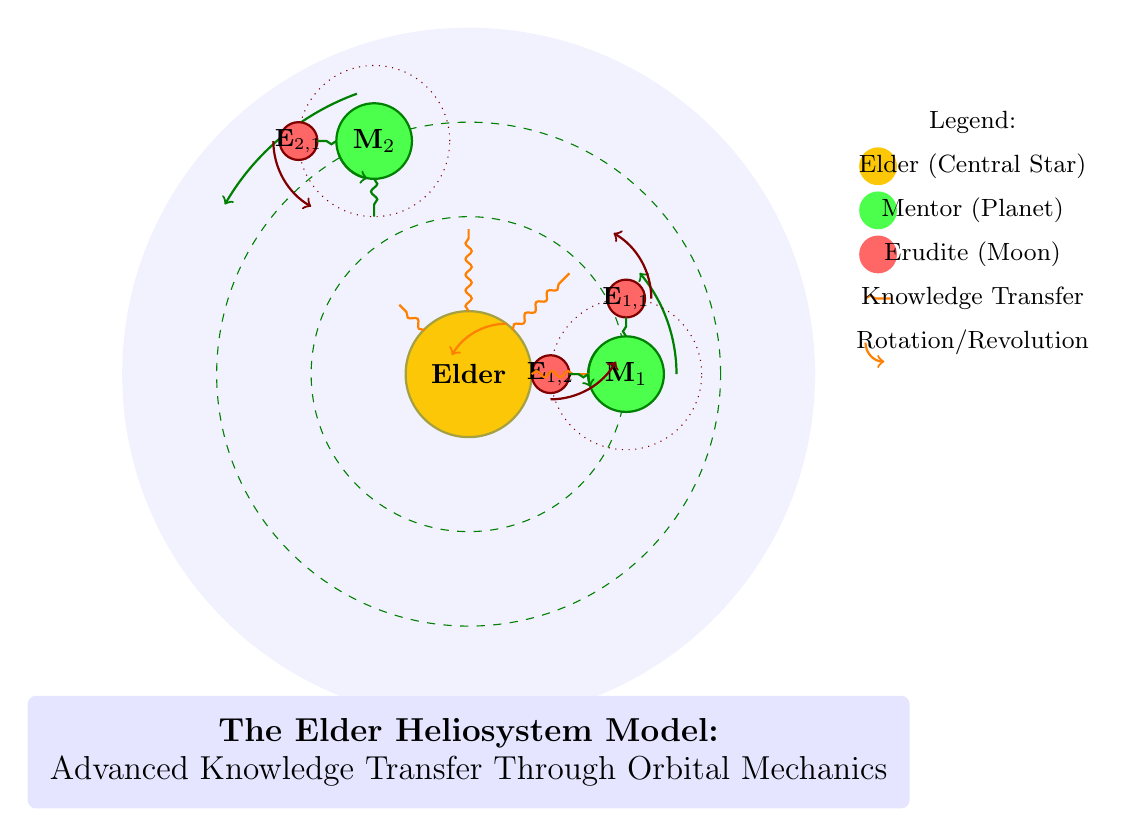
\begin{tikzpicture}[scale=0.8,
  decoration={snake, amplitude=.4mm, segment length=2mm, post length=1mm}
]
  % Draw background
  \fill[blue!5] (0,0) circle (5.5);
  
  % Draw Elder (Sun)
  \fill[yellow!80!red] (0,0) circle (1);
  \draw[yellow!60!black, thick] (0,0) circle (1);
  \node at (0,0) {\textbf{Elder}};
  
  % Draw rotational indicator for Elder
  \draw[->, thick, orange] (0.6,0.8) arc (90:150:1);
  
  % Draw Mentor1 orbit
  \draw[green!50!black, dashed] (0,0) circle (2.5);
  
  % Draw Mentor2 orbit
  \draw[green!50!black, dashed] (0,0) circle (4);
  
  % Draw Mentor1 (Planet)
  \fill[green!70] (2.5,0) circle (0.6);
  \draw[green!50!black, thick] (2.5,0) circle (0.6);
  \node at (2.5,0) {\textbf{M$_1$}};
  
  % Draw Mentor2 (Planet)
  \fill[green!70] (-1.5,3.7) circle (0.6);
  \draw[green!50!black, thick] (-1.5,3.7) circle (0.6);
  \node at (-1.5,3.7) {\textbf{M$_2$}};
  
  % Draw rotational indicators for Mentors
  \draw[->, thick, green!50!black] (2.5,0) + (140:0.6) arc (140:200:0.6);
  \draw[->, thick, green!50!black] (-1.5,3.7) + (200:0.6) arc (200:260:0.6);
  
  % Draw Mentor1 orbital direction
  \draw[->, thick, green!50!black] (2.5,0) + (0:0.8) arc (0:40:2.5);
  
  % Draw Mentor2 orbital direction
  \draw[->, thick, green!50!black] (-1.5,3.7) + (110:0.8) arc (110:150:4);
  
  % Draw Erudite orbits around Mentor1
  \draw[red!50!black, dotted] (2.5,0) circle (1.2);
  
  % Draw Erudites (Moons) around Mentor1
  \fill[red!60] (2.5,1.2) circle (0.3);
  \draw[red!50!black, thick] (2.5,1.2) circle (0.3);
  \node at (2.5,1.2) {\textbf{\small E$_{1,1}$}};
  
  \fill[red!60] (1.3,0) circle (0.3);
  \draw[red!50!black, thick] (1.3,0) circle (0.3);
  \node at (1.3,0) {\textbf{\small E$_{1,2}$}};
  
  % Draw Erudite orbit around Mentor2
  \draw[red!50!black, dotted] (-1.5,3.7) circle (1.2);
  
  % Draw Erudite (Moon) around Mentor2
  \fill[red!60] (-2.7,3.7) circle (0.3);
  \draw[red!50!black, thick] (-2.7,3.7) circle (0.3);
  \node at (-2.7,3.7) {\textbf{\small E$_{2,1}$}};
  
  % Draw orbital direction for Erudites
  \draw[->, thick, red!50!black] (2.5,1.2) + (0:0.4) arc (0:60:1.2);
  \draw[->, thick, red!50!black] (1.3,0) + (270:0.4) arc (270:330:1.2);
  \draw[->, thick, red!50!black] (-2.7,3.7) + (180:0.4) arc (180:240:1.2);
  
  % Draw Elder field propagation (wave)
  \draw[orange, decorate, thick] (1,0) -- (1.9,0);
  \draw[orange, decorate, thick] (0.7,0.7) -- (1.6,1.6);
  \draw[orange, decorate, thick] (0,1) -- (0,2.3);
  \draw[orange, decorate, thick] (-0.7,0.7) -- (-1.1,1.1);
  
  % Draw mentor field propagation (wave)
  \draw[green!50!black, decorate, thick] (2.5,0.6) -- (2.5,0.9);
  \draw[green!50!black, decorate, thick] (1.9,0) -- (1.6,0);
  \draw[green!50!black, decorate, thick] (-1.5,3.1) -- (-1.5,2.5);
  \draw[green!50!black, decorate, thick] (-2.1,3.7) -- (-2.4,3.7);
  
  % Draw labels
  \node[font=\large, align=center, fill=blue!10, rounded corners=3pt, inner sep=8pt] at (0,-6) {\textbf{The Elder Heliosystem Model:}\\Advanced Knowledge Transfer Through Orbital Mechanics};
  
  % Draw legend
  \node[font=\small, align=left] at (8,4) {Legend:};
  \fill[yellow!80!red] (6.5,3.3) circle (0.3);
  \node[font=\small, align=left] at (8,3.3) {Elder (Central Star)};
  \fill[green!70] (6.5,2.6) circle (0.3);
  \node[font=\small, align=left] at (8,2.6) {Mentor (Planet)};
  \fill[red!60] (6.5,1.9) circle (0.3);
  \node[font=\small, align=left] at (8,1.9) {Erudite (Moon)};
  \draw[orange, decorate, thick] (6.3,1.2) -- (6.7,1.2);
  \node[font=\small, align=left] at (8,1.2) {Knowledge Transfer};
  \draw[->, thick, orange] (6.3,0.5) arc (180:270:0.3);
  \node[font=\small, align=left] at (8,0.5) {Rotation/Revolution};
\end{tikzpicture}
\caption{The Elder Heliosystem model illustrating the heliocentric approach to knowledge transfer. Elder (center) represents the source of universal principles, Mentors (planets) represent domain-specific knowledge, and Erudites (moons) represent task-specific knowledge. The transfer of information is mediated through orbital dynamics, with frequency synchronization determining the efficiency of knowledge flow.}
\label{fig:elder_heliosystem}
\end{figure}

\section{Applications to Enriched Audio Generation}

The Elder framework is particularly well-suited for generating enriched audio data with complex spatial and temporal characteristics.

\begin{example}
Consider an application to spatial audio synthesis for virtual environments. The Erudite component learns to generate audio based on environmental parameters, the Mentor component provides guidance on how spatial audio should be distributed given the environment's geometry, and the Elder component ensures consistency of physical audio principles across different scenarios through tensor embeddings that encode acoustic laws.
\end{example}

\begin{theorem}[Generalization Bound]
For an Elder-Mentor-Erudite system trained on dataset $\mathcal{D}$ with $|\mathcal{D}| = n$ samples, with probability at least $1-\delta$, the expected Elder Loss on unseen data satisfies:
\begin{equation}
\mathbb{E}[\eloss] \leq \frac{1}{n}\sum_{i=1}^n \eloss(\theta_M, \theta_E, x_i, y_i) + \mathcal{O}\left(\sqrt{\frac{\log(1/\delta)}{n}}\right) \cdot R(\mathcal{T})
\end{equation}
where $R(\mathcal{T})$ is a complexity measure of the tensor embedding function, specifically defined as:
\begin{equation}
R(\mathcal{T}) = \sqrt{\text{rank}(\mathcal{T})} \cdot \log(\|\mathcal{T}\|_{\text{op}}) \cdot \mathcal{C}_{\text{phase}}(\mathcal{T})
\end{equation}
with $\text{rank}(\mathcal{T})$ being the tensor rank, $\|\mathcal{T}\|_{\text{op}}$ the operator norm, and $\mathcal{C}_{\text{phase}}(\mathcal{T}) = \int_0^{2\pi} |\mathcal{T}(e^{i\phi})|^2 d\phi$ measuring phase coherence complexity.
\end{theorem}

\section{Connection to Algebraic Structure}

The Elder Loss establishes a deeper connection to the algebraic structure of Elder spaces through its tensor embeddings. This section explores the profound algebraic foundations of the Elder framework, revealing how the hierarchical learning system inherits rich mathematical structures that enable its cross-domain knowledge transfer capabilities.

\subsection{Induced Algebraic Operations}

\begin{proposition}
The tensor embedding function $\mathcal{T}$ induces a non-commutative product $\star$ on the parameter space such that for $\theta_1, \theta_2 \in \paramspace = \mentorparams \times \eruditeparams$:
\begin{equation}
\mathcal{T}(\theta_1 \star \theta_2) = \mathcal{T}(\theta_1) \bullet \mathcal{T}(\theta_2)
\end{equation}
where $\bullet$ denotes a tensor contraction operation.
\end{proposition}

\begin{proof}
Let the tensor embedding $\mathcal{T}: \paramspace \rightarrow \mathbb{R}^{d_1 \times d_2 \times \cdots \times d_k}$ map parameters to $k$-dimensional tensors. We can construct the non-commutative product $\star: \paramspace \times \paramspace \rightarrow \paramspace$ as:
\begin{equation}
\theta_1 \star \theta_2 = \mathcal{T}^{-1}(\mathcal{T}(\theta_1) \bullet \mathcal{T}(\theta_2))
\end{equation}
where $\mathcal{T}^{-1}$ represents a pseudo-inverse mapping from the tensor space back to parameter space. The operation $\bullet$ is defined as a specific tensor contraction that preserves the hierarchical relationships between parameters. The non-commutativity follows from the directional nature of knowledge transfer in the Elder-Mentor-Erudite hierarchy.
\end{proof}

\begin{definition}[Elder Algebra]
The parameter space $\paramspace = \mentorparams \times \eruditeparams$ equipped with the non-commutative product $\star$ forms an algebra $(\paramspace, +, \star, \cdot)$ where $+$ denotes parameter addition, $\star$ is the induced product, and $\cdot$ is scalar multiplication. This structure is called the Elder Algebra.
\end{definition}

\begin{theorem}[Elder Space Isomorphism]
The unified parameter space $\paramspace = \mentorparams \times \eruditeparams$ equipped with the non-commutative product $\star$ is isomorphic to a subspace of the singular Elder space $\elder{d}$ under the mapping $\mathcal{T}$.
\end{theorem}

\begin{proof}
We need to establish that $\mathcal{T}$ preserves both algebraic operations and structural relationships. For addition:
\begin{equation}
\mathcal{T}(\theta_1 + \theta_2) = \mathcal{T}(\theta_1) \oplus \mathcal{T}(\theta_2)
\end{equation}
where $\oplus$ represents a suitable tensor addition operation. The tensor embedding $\mathcal{T}$ further preserves the scalar multiplication:
\begin{equation}
\mathcal{T}(\alpha \cdot \theta) = \alpha \otimes \mathcal{T}(\theta)
\end{equation}
And as established in the previous proposition, $\mathcal{T}$ preserves the non-commutative product $\star$. Since $\mathcal{T}$ preserves all algebraic operations and is injective by construction, it establishes an isomorphism between $(\paramspace, +, \star, \cdot)$ and a subspace of $\elder{d}$.
\end{proof}

\subsection{Hierarchical Space Projections}

\begin{corollary}[Space Hierarchy]
The multiple Mentor spaces $\{\mathcal{M}_1, \mathcal{M}_2, \ldots, \mathcal{M}_m\}$ and Erudite spaces $\{\mathcal{E}_1, \mathcal{E}_2, \ldots, \mathcal{E}_n\}$ are all projected into distinct regions of the singular Elder space $\elder{d}$ via the tensor embedding function $\mathcal{T}$, forming a hierarchical structure where:
\begin{equation}
\mathcal{E}_j \subset \mathcal{M}_i \subset \elder{d}
\end{equation}
for each Erudite space $\mathcal{E}_j$ associated with a Mentor space $\mathcal{M}_i$.
\end{corollary}

\begin{definition}[Projection Operators]
For each Mentor space $\mathcal{M}_i$ and associated Erudite spaces $\{\mathcal{E}_{i1}, \mathcal{E}_{i2}, \ldots\}$, we define projection operators:
\begin{align}
\Pi_{\mathcal{M}_i}: \elder{d} &\rightarrow \mathcal{M}_i \\
\Pi_{\mathcal{E}_{ij}}: \mathcal{M}_i &\rightarrow \mathcal{E}_{ij}
\end{align}
that extract domain-specific and task-specific knowledge from the Elder space.
\end{definition}

\begin{proposition}[Projection Properties]
The projection operators satisfy:
\begin{align}
\Pi_{\mathcal{M}_i} \circ \Pi_{\mathcal{M}_i} &= \Pi_{\mathcal{M}_i} \quad \text{(idempotence)}\\
\Pi_{\mathcal{E}_{ij}} \circ \Pi_{\mathcal{E}_{ij}} &= \Pi_{\mathcal{E}_{ij}} \quad \text{(idempotence)}\\
\Pi_{\mathcal{E}_{ij}} \circ \Pi_{\mathcal{M}_i} &= \Pi_{\mathcal{E}_{ij}} \quad \text{(composition)}
\end{align}
Furthermore, for distinct domains $i \neq i'$, the projections have minimal interference:
\begin{equation}
\| \Pi_{\mathcal{M}_i} \circ \Pi_{\mathcal{M}_{i'}} \|_F \leq \epsilon \quad \text{for some small } \epsilon > 0
\end{equation}
\end{proposition}

\subsection{Lie Group Structure in Parameter Transformations}

The Elder framework's parameter transformations during learning exhibit rich geometric structures that can be understood through Lie group theory.

\begin{theorem}[Elder Lie Group]
The continuous transformations of Elder parameters form a Lie group $G_E$ acting on the Elder space $\elder{d}$, with the Lie algebra $\mathfrak{g}_E$ characterizing infinitesimal parameter updates during gradient-based learning.
\end{theorem}

\begin{proof}[Sketch]
Consider the continuous family of transformations $\{\phi_t\}_{t \in \mathbb{R}}$ where $\phi_t: \elder{d} \rightarrow \elder{d}$ represents parameter updates after $t$ units of training time. These transformations satisfy:
\begin{enumerate}
\item $\phi_0$ is the identity transformation
\item $\phi_s \circ \phi_t = \phi_{s+t}$ (group property)
\item The mapping $(t, \theta) \mapsto \phi_t(\theta)$ is smooth
\end{enumerate}
Therefore, $\{\phi_t\}$ forms a one-parameter subgroup of the Lie group $G_E$. The generator of this subgroup corresponds to the gradient of the Elder Loss, which resides in the Lie algebra $\mathfrak{g}_E$.
\end{proof}

\begin{corollary}[Manifold Structure]
The optimal parameter configurations for different domains form a smooth manifold $\mathcal{M} \subset \elder{d}$ with the Lie group $G_E$ acting transitively on connected components of $\mathcal{M}$.
\end{corollary}

\subsection{Information Geometry Perspective}

The Elder space can also be understood through the lens of information geometry, which provides powerful tools for analyzing the hierarchical learning dynamics.

\begin{definition}[Fisher Information Metric]
The Fisher information metric $g_{ij}$ on the parameter space $\paramspace$ is defined as:
\begin{equation}
g_{ij}(\theta) = \mathbb{E}_{x,y \sim \mathcal{D}}\left[ \frac{\partial \eloss(\theta, x, y)}{\partial \theta^i} \frac{\partial \eloss(\theta, x, y)}{\partial \theta^j} \right]
\end{equation}
This metric defines a Riemannian geometry on the parameter space.
\end{definition}

\begin{theorem}[Information Geometric Structure]
The Elder space $\elder{d}$ equipped with the Fisher information metric forms a statistical manifold where:
\begin{enumerate}
\item Geodesics correspond to optimal paths for parameter transfer between domains
\item The divergence between parameter configurations measures the difficulty of knowledge transfer
\item The curvature of the manifold characterizes the nonlinearity of the learning dynamics
\end{enumerate}
\end{theorem}

\begin{proposition}[Hierarchical Geodesic Flow]
The gradient flow of the Elder Loss follows a path that approximates geodesics in the information geometric manifold, with corrections due to the tensor embedding structure:
\begin{equation}
\frac{d\theta}{dt} = -g^{ij}(\theta) \frac{\partial \eloss}{\partial \theta^j} + \Gamma^i_{jk}(\theta) \theta^j \theta^k
\end{equation}
where $g^{ij}$ is the inverse Fisher metric and $\Gamma^i_{jk}$ are the Christoffel symbols of the Levi-Civita connection.
\end{proposition}

This connection completes the circle of our theoretical development, showing how the concepts of Elder Loss, Mentor Loss, and Erudite Loss are intricately related to the algebraic and geometric structures of Elder spaces that we developed in earlier chapters. The algebraic perspective provides a principled foundation for understanding the hierarchical knowledge representation and transfer mechanisms that enable the Elder framework's remarkable cross-domain generalization capabilities.

\section{Task Generalization and Training Methodology}

A key advantage of the Elder-Mentor-Erudite framework is its ability to generalize across different tasks while accumulating knowledge.

\begin{definition}[Task Space]
Let $\mathcal{T}$ be a task space, where each task $\tau \in \mathcal{T}$ is defined by a data distribution $\mathcal{D}_\tau$ and a task-specific loss function $\ell_\tau: \mathcal{Y} \times \mathcal{Y} \rightarrow \mathbb{R}_+$.
\end{definition}

\begin{theorem}[Erudite Adaptability]
Given a trained Erudite with parameters $\theta_E$ and a new task $\tau_{\text{new}} \in \mathcal{T}$, the adaptation process can be formulated as:
\begin{equation}
\theta_E^{\tau_{\text{new}}} = \theta_E - \eta \nabla_{\theta_E} \erloss(x, y; \theta_E, \tau_{\text{new}})
\end{equation}
where $\eta > 0$ is a learning rate, and the task-specific Erudite Loss is defined as:
\begin{equation}
\erloss(x, y; \theta_E, \tau) = \| \mathcal{F}_\tau(y) - \mathcal{F}_\tau(\hat{y}) \|_{\mathcal{H}}^2 + \lambda_E \cdot \ell_\tau(y, \hat{y})
\end{equation}
\end{theorem}

\begin{proposition}[Mentor Knowledge Accumulation]
As Mentor guides Erudite through multiple tasks $\tau_1, \tau_2, \ldots, \tau_n$, its parameters $\theta_M$ evolve according to:
\begin{equation}
\theta_M^{(n)} = \theta_M^{(n-1)} - \gamma \nabla_{\theta_M} \mloss(\theta_E^{\tau_n}, \mathcal{D}_{\tau_n}; \theta_M^{(n-1)})
\end{equation}
where $\gamma > 0$ is the Mentor learning rate. This process accumulates teaching knowledge across diverse tasks.
\end{proposition}

\begin{definition}[Space Production]
Within the Elder-Mentor-Erudite framework:
\begin{enumerate}
    \item \textbf{Elder Space}: A singular, unified space $\elder{d}$ governed by a single Elder model that establishes global principles.
    \item \textbf{Mentor Spaces}: Multiple spaces $\{\mathcal{M}_1, \mathcal{M}_2, \ldots, \mathcal{M}_m\}$ where each $\mathcal{M}_i \subset \mentorparams$ represents a specialized teaching strategy for a family of related tasks.
    \item \textbf{Erudite Spaces}: Multiple task-specific spaces $\{\mathcal{E}_1, \mathcal{E}_2, \ldots, \mathcal{E}_n\}$ where each $\mathcal{E}_j \subset \eruditeparams$ contains parameters optimized for executing specific tasks.
\end{enumerate}
\end{definition}

\begin{definition}[Training Protocol]
The Elder-Mentor-Erudite training protocol consists of three nested optimization loops:
\begin{enumerate}
    \item \textbf{Inner Loop (Erudite)}: For fixed Mentor parameters $\theta_M$, optimize Erudite parameters $\theta_E$ on task $\tau$ to minimize $\erloss$, producing task-specific Erudite spaces.
    \item \textbf{Middle Loop (Mentor)}: Update Mentor parameters $\theta_M$ based on Erudite's performance to minimize $\mloss$, generating specialized Mentor spaces for different task families.
    \item \textbf{Outer Loop (Elder)}: An indefinitely running process that continuously adjusts the tensor embedding function $\mathcal{T}$ to ensure consistency across all Mentor and Erudite spaces while minimizing $\eloss$.
\end{enumerate}
\end{definition}

\begin{proposition}[Continual Elder Optimization]
The Elder optimization process is designed to run indefinitely, with its tensor embedding function $\mathcal{T}$ evolving according to:
\begin{equation}
\mathcal{T}_{t+1} = \mathcal{T}_t - \lambda \nabla_{\mathcal{T}} \eloss(\Theta_M^t, \Theta_E^t, \mathcal{D}^t)
\end{equation}
where $\Theta_M^t$ and $\Theta_E^t$ represent the collective Mentor and Erudite parameter spaces at time $t$, $\mathcal{D}^t$ is the accumulated dataset of all tasks encountered up to time $t$, and $\lambda > 0$ is the Elder learning rate.
\end{proposition}

\begin{example}[Domain-Specific Learning: Audio Generation]
Consider training the system on the audio generation domain with multiple tasks:
\begin{itemize}
    \item $\tau_1$: Speech synthesis for a specific language
    \item $\tau_2$: Environmental sound generation
    \item $\tau_3$: Musical instrument simulation
\end{itemize}
This represents just one domain among many that the Elder-Mentor-Erudite system can master, with other potential domains including computer vision, language understanding, mathematical reasoning, molecular design, robotic control, and many others.
\end{example}

\subsection{Task-Specific Learning in Erudite}

The Erudite component serves as the task-specific executor in the Elder-Mentor-Erudite framework. For each distinct audio generation task, a specialized Erudite space emerges through training.

\begin{definition}[Task-Specific Erudite Space]
For each task $\tau_i$, a dedicated Erudite space $\mathcal{E}_i \subset \eruditeparams$ develops, characterized by:
\begin{equation}
\mathcal{E}_i = \{\theta_E \in \eruditeparams \mid \erloss(x, y; \theta_E, \tau_i) < \epsilon_i \text{ for } (x,y) \sim \mathcal{D}_{\tau_i}\}
\end{equation}
where $\epsilon_i > 0$ is a task-specific error threshold.
\end{definition}

For instance, in speech synthesis ($\tau_1$), Erudite learns specific phonetic representations, prosodic patterns, and speaker characteristics. Its parameters encode task-specific knowledge like:
\begin{itemize}
    \item Phoneme-to-acoustic mapping matrices
    \item Temporal alignment patterns for natural speech rhythms
    \item Speaker-dependent vocal tract parameters
\end{itemize}

Similarly, for environmental sound generation ($\tau_2$), Erudite develops distinct parameter configurations for modeling physical sound propagation, material properties, and spatial characteristics of environments.

\begin{proposition}[Erudite Specialization]
As training progresses on task $\tau_i$, the corresponding Erudite parameters $\theta_E^{\tau_i}$ increasingly specialize, forming a distinct manifold $\mathcal{E}_i$ in parameter space that optimizes performance exclusively for that task.
\end{proposition}

\subsection{Domain-Specific Meta-Knowledge Accumulation in Mentor}

While Erudite specializes in task execution, the Mentor component accumulates meta-knowledge—knowledge about how to teach Erudite to perform various tasks efficiently within a specific domain.

\begin{definition}[Mentor Knowledge Space]
For a family of related tasks $\{\tau_1, \tau_2, \ldots, \tau_k\}$ within domain $D$, a Mentor knowledge space $\mathcal{M}_j^D \subset \mentorparams$ forms, characterized by:
\begin{equation}
\mathcal{M}_j^D = \{\theta_M \in \mentorparams \mid \mloss(\theta_E, \mathcal{D}_{\tau_i}; \theta_M) < \delta_j \text{ for all } i \in \{1,2,\ldots,k\}\}
\end{equation}
where $\delta_j > 0$ is a meta-knowledge quality threshold.
\end{definition}

The Mentor's accumulated domain-specific knowledge includes:
\begin{itemize}
    \item Cross-task feature transfer mappings that identify reusable domain primitives
    \item Optimization trajectory templates that efficiently guide parameter updates for domain-specific tasks
    \item Task decomposition strategies that break complex tasks into manageable subtasks appropriate for the domain
    \item Difficulty progression schedules that sequence learning from simple to complex patterns within the domain
\end{itemize}

\begin{theorem}[Domain-Specific Mentor Knowledge Transfer]
A well-trained Mentor with parameters $\theta_M \in \mathcal{M}_j^D$ can guide an untrained Erudite to learn a new task $\tau_{new}$ within domain $D$ with significantly fewer examples than learning from scratch, bounded by:
\begin{equation}
|\mathcal{D}_{\tau_{new}}^{\text{required}}| \leq \rho \cdot \min_i |\mathcal{D}_{\tau_i}^{\text{required}}| \cdot \left(1 - \frac{\text{MI}(\tau_{new}; \{\tau_1,\ldots,\tau_k\})}{\text{H}(\tau_{new})}\right)
\end{equation}
where $\text{MI}$ is mutual information, $\text{H}$ is entropy, and $\rho > 0$ is a constant.
\end{theorem}

\subsection{Universal Principle Accumulation in Elder}

The Elder component operates as a singular, distinct entity at the highest level of abstraction, learning directly from the manifold produced by the learned parameters of all Mentors across different domains, and accumulating universal principles that transcend domain boundaries.

\begin{definition}[Elder Knowledge]
Elder knowledge consists of a set of universal principles $\Pi = \{\pi_1, \pi_2, \ldots, \pi_n\}$ that transcend specific domains, where each $\pi_i$ represents a fundamental pattern, law, or structure that applies across diverse fields of knowledge, derived from the parameter manifolds of domain-specific Mentors.
\end{definition}

Unlike Mentor which accumulates knowledge about teaching specific task domains (e.g., audio generation, image processing, language modeling), Elder is an entirely separate entity that learns from the collective manifold of all Mentor parameters, distilling higher-order principles that apply universally, such as:
\begin{itemize}
    \item Conservation laws that manifest across physical, computational, and mathematical domains
    \item Hierarchical compositional structures common to all complex systems
    \item Information-theoretic limits that constrain any learning process
    \item Causality and temporal dependence patterns that appear in diverse domains
    \item Symmetry and invariance properties that generalize across modalities
    \item Transfer principles that govern knowledge mapping between seemingly unrelated domains
\end{itemize}

\begin{theorem}[Elder Domain-Bridging]
For any two distinct domains $D_1$ and $D_2$ with corresponding Mentor spaces $\mathcal{M}_1$ and $\mathcal{M}_2$, Elder establishes a mapping $\Gamma: \mathcal{M}_1 \times \mathcal{M}_2 \rightarrow \elder{d}$ such that:
\begin{equation}
\text{MI}(D_1; D_2 | \Gamma) > \text{MI}(D_1; D_2)
\end{equation}
where $\text{MI}$ is mutual information, indicating that Elder increases the information shared between domains by identifying underlying universal principles.
\end{theorem}

\begin{example}
When Elder observes both audio generation and mathematical theorem proving, it might discover that the principle of compositional structure—building complex outcomes from simpler components—applies in both domains. In audio, this manifests as combining fundamental waveforms to create complex sounds; in theorem proving, it appears as combining lemmas to build proofs.
\end{example}

\begin{proposition}[Magnitude-Higher Learning]
As a magnitude-higher learning system, Elder's parameter space dimensionality relates to Mentor's through:
\begin{equation}
\dim(\elder{d}) \approx \mathcal{O}(\dim(\mentorparams)^{\alpha})
\end{equation}
where $\alpha > 1$ reflects the higher-order abstraction capability of Elder.
\end{proposition}

\begin{definition}[Elder Learning from Mentor Manifolds]
Let $\mathcal{M} = \{\mathcal{M}_1^{D_1}, \mathcal{M}_2^{D_2}, \ldots, \mathcal{M}_k^{D_k}\}$ be the set of all Mentor parameter manifolds across different domains. Elder learns directly from this collective manifold through:
\begin{equation}
\elderloss(\mathcal{M}; \elderparam) = \mathbb{E}_{(\mathcal{M}_i^{D_i}, \mathcal{M}_j^{D_j}) \sim \mathcal{M}^2} \left[ d\left(\Phi(\mathcal{M}_i^{D_i}, \mathcal{M}_j^{D_j}; \elderparam), \mathcal{R}(D_i, D_j)\right) \right]
\end{equation}
where $\Phi$ is Elder's cross-domain mapping function, $\mathcal{R}(D_i, D_j)$ represents the true underlying relationships between domains, and $d$ is a distance metric in the space of cross-domain relationships.
\end{definition}

\subsection{Complex Space Representation and Self-Reflection Manifold}

A critical and distinctive feature of Elder is its operation within complex vector spaces, enabling richer representations of cross-domain principles through phase information and complex-valued transformations.

\begin{definition}[Complex Parameter Space]
Elder's parameters exist in a complex Hilbert space $\celderparams$, with each parameter $\theta_{\text{Elder}} \in \complex^n$ rather than $\mathbb{R}^n$ as in Mentor and Erudite systems.
\end{definition}

\begin{theorem}[Complex Domain Encoding]
For any domain $D_i$ with corresponding Mentor manifold $\mathcal{M}_i^{D_i}$, Elder constructs a complex embedding through:
\begin{equation}
\complexmap: \mathcal{M}_i^{D_i} \rightarrow \complexn{d}
\end{equation}
where both magnitude and phase encode semantically meaningful domain properties:
\begin{equation}
\complexmap(\mathcal{M}_i^{D_i}) = r_i(\mathcal{M}_i^{D_i})e^{j\phi_i(\mathcal{M}_i^{D_i})}
\end{equation}
with $r_i$ encoding domain robustness and $\phi_i$ encoding domain relationships.
\end{theorem}

\begin{definition}[Self-Reflection Manifold]
Elder forms a self-reflection manifold $\selfmanifold \subset \complexn{d \times d}$ through hermitian outer products of complex domain encodings:
\begin{equation}
\selfmanifold_{i,j} = \complexmap(\mathcal{M}_i^{D_i}) \cdot \hermitian{\complexmap(\mathcal{M}_j^{D_j})}
\end{equation}
which forms a complex manifold structure encoding both intra-domain and inter-domain relationships.
\end{definition}

\subsection{Kernel-Level Operations}

The computational core of Elder operates through specialized complex-valued kernel operations designed for accelerator devices.

\begin{definition}[Elder Kernel]
The fundamental kernel operation $\elkernel: \complex^n \times \complex^m \rightarrow \complex^{n \times m}$ is defined as:
\begin{equation}
\elkernel(\mathbf{x}, \mathbf{y}; \elderparam) = \sigma\left(\sum_{l=1}^L W_l \cdot (\mathbf{x} \otimes \hermitian{\mathbf{y}}) \cdot \hermitian{W_l}\right)
\end{equation}
where $\otimes$ is the outer product, $W_l \in \complex^{n \times m}$ are learnable complex weight matrices, and $\sigma$ is a complex activation function preserving holomorphicity in regions of interest.
\end{definition}

The complex-valued kernel enables exponentially more representational capacity than real-valued operations through:

\begin{itemize}
    \item \textbf{Phase Coherence Detection:} Measuring alignment of principles across domains through complex phase relationships
    \item \textbf{Interference Pattern Recognition:} Identifying constructive and destructive interference between domain principles
    \item \textbf{Holomorphic Constraint Satisfaction:} Enforcing mathematical consistency through complex differentiability
    \item \textbf{Quantum-Inspired Entanglement:} Modeling inseparable relationships between domain principles
\end{itemize}

\begin{theorem}[Kernel Acceleration Complexity]
The Elder kernel operation achieves acceleration through decomposition into parallel streams, with time complexity:
\begin{equation}
T(\elkernel) = \mathcal{O}\left(\frac{n \cdot m \cdot L}{p}\right)
\end{equation}
where $p$ is the number of parallel processing elements in the accelerator device.
\end{theorem}

\begin{proposition}[Kernel Factorization]
The Elder kernel operation can be factorized for efficient implementation on specialized hardware through:
\begin{equation}
\elkernel(\mathbf{x}, \mathbf{y}; \elderparam) = \sum_{l=1}^L \sigma_l\left(U_l \cdot \mathbf{x}\right) \otimes \sigma_l\left(V_l \cdot \mathbf{y}^*\right)
\end{equation}
where $U_l \in \complex^{d' \times n}$, $V_l \in \complex^{d' \times m}$ are low-rank factorizations of $W_l$, $\mathbf{y}^*$ is the complex conjugate of $\mathbf{y}$, and $\sigma_l$ are complex nonlinearities.
\end{proposition}

\subsection{Low-Level Kernel Implementation with Go and OpenCL}

The Elder kernel is implemented using Go as the primary language, with computation-intensive operations offloaded to accelerator devices via OpenCL. This architecture leverages Go's concurrency model while harnessing the computational power of GPUs and other specialized hardware.

\begin{center}
\textbf{Elder Kernel Implementation in Go with OpenCL}
\end{center}

\begin{verbatim}
// Go implementation of Elder kernel using OpenCL
// Package elder/kernel/cl.go

package kernel

import (
    "github.com/go-gl/cl/v1.2/cl"
    "github.com/elder/tensor"
    "github.com/elder/complex"
)

// OpenCL kernel source for complex operations
const elderKernelSource = `
    // Complex number operations in OpenCL
    typedef struct { float real; float imag; } complex_t;
    
    // Hermitian outer product kernel
    __kernel void hermitianOuterProduct(
        __global const complex_t* x,
        __global const complex_t* y,
        __global complex_t* result,
        const int n,
        const int m
    ) {
        int i = get_global_id(0);
        int j = get_global_id(1);
        
        if (i < n && j < m) {
            // z = x[i] * conj(y[j])
            complex_t z;
            z.real = x[i].real * y[j].real + x[i].imag * y[j].imag;
            z.imag = x[i].imag * y[j].real - x[i].real * y[j].imag;
            
            result[i*m + j] = z;
        }
    }
    
    // Complex matrix multiplication with weights
    __kernel void complexMatrixMultiply(
        __global const complex_t* weights,
        __global const complex_t* input,
        __global complex_t* output,
        const int n,
        const int m
    ) {
        // Matrix multiplication implementation
        // ...
    }
    
    // Holomorphic activation function
    __kernel void complexActivation(
        __global complex_t* data,
        const int size
    ) {
        int idx = get_global_id(0);
        if (idx < size) {
            // Complex-valued activation preserving holomorphicity
            // Using Taylor series expansion of holomorphic function
            // ...
        }
    }
`;

// ElderKernel executes the complex operations on OpenCL device
func ElderKernel(x, y, weights *tensor.ComplexTensor, n, m, l int) (*tensor.ComplexTensor, error) {
    // Initialize OpenCL
    platforms, err := cl.GetPlatforms()
    if err != nil {
        return nil, err
    }
    
    // Select platform and device
    devices, err := platforms[0].GetDevices(cl.DeviceTypeAll)
    if err != nil {
        return nil, err
    }
    
    // Create context, command queue, and program
    context, err := cl.CreateContext([]*cl.Device{devices[0]}, nil, nil)
    if err != nil {
        return nil, err
    }
    defer context.Release()
    
    queue, err := context.CreateCommandQueue(devices[0], 0)
    if err != nil {
        return nil, err
    }
    defer queue.Release()
    
    program, err := context.CreateProgramWithSource([]string{elderKernelSource})
    if err != nil {
        return nil, err
    }
    
    // Build program
    if err := program.BuildProgram(nil, ""); err != nil {
        return nil, err
    }
    
    // Allocate and transfer memory
    result := tensor.NewComplexTensor(n, m)
    
    // Execute kernels
    // ... (Create and execute kernels for each operation)
    
    return result, nil
}
\end{verbatim}

\begin{proposition}[Memory Access Optimization]
The Elder kernel minimizes global memory access through block-wise operations that maximize data locality:
\begin{equation}
\text{Memory Accesses} = \mathcal{O}(B_n \cdot B_m + n \cdot m)
\end{equation}
where $B_n$ and $B_m$ are block sizes chosen to optimize cache utilization.
\end{proposition}

\subsection{Go and OpenCL in the Elder Architecture}

The implementation of Elder using Go as the high-level language and OpenCL for accelerator computations offers several advantages that align with Elder's mission of cross-domain knowledge integration:

\begin{itemize}
    \item \textbf{Concurrency Model}: Go's goroutines enable efficient management of multiple concurrent Mentor training processes, allowing Elder to simultaneously observe and learn from diverse domains.
    
    \item \textbf{Heterogeneous Computing}: OpenCL provides access to GPUs, FPGAs, and specialized AI accelerators, enabling efficient execution of complex-valued operations across diverse hardware.
    
    \item \textbf{Memory Management}: Go's garbage collection combined with OpenCL's explicit memory model allows Elder to efficiently manage both long-term knowledge storage and temporary computational buffers.
    
    \item \textbf{Abstraction Layers}: The system implements three abstraction layers:
    \begin{enumerate}
        \item Go domain logic for high-level reasoning and system coordination
        \item Intermediate tensor manipulation for data preparation and result interpretation
        \item Low-level OpenCL kernels for maximum computational efficiency in complex-valued operations
    \end{enumerate}
\end{itemize}

The Elder system dynamically manages workload distribution between CPU-bound Go code and GPU-accelerated OpenCL kernels. This hybrid approach allows for flexibility in deployment scenarios, from high-end servers with multiple GPUs to more modest computing environments, with the system automatically adapting to available resources.

The indefinite optimization process of Elder continuously refines its tensor embedding function $\mathcal{T}$ and complex mappings to better capture universal principles across all domains it encounters by analyzing the self-reflection manifold structure derived from all Mentor parameters. This allows Elder to guide Mentors in new domains with increasingly abstract and generalized knowledge, even when those domains appear entirely unrelated to previously encountered ones.

\begin{theorem}[Elder Cross-Domain Consistency]
For any two Mentors $\theta_M^i \in \mathcal{M}_i$ and $\theta_M^j \in \mathcal{M}_j$ operating in different domains, the Elder tensor embedding $\mathcal{T}$ ensures that:
\begin{equation}
\| \Pi_{\Pi}(\mathcal{T}(\theta_M^i)) - \Pi_{\Pi}(\mathcal{T}(\theta_M^j)) \|_F < \epsilon_{univ}
\end{equation}
where $\Pi_{\Pi}$ is a projection onto the subspace of universal principles $\Pi$, and $\epsilon_{univ} > 0$ is a consistency tolerance for universal knowledge.
\end{theorem}

This hierarchical structure creates a comprehensive framework where Erudite maintains task-specific proficiency, Mentor accumulates domain-specific teaching knowledge, and Elder—as a distinct entity that learns from the parameter manifolds of all Mentors—distills universal principles that bridge across all domains, enabling truly general intelligence that transcends domain boundaries.

\begin{theorem}[Transfer Efficiency]
If the Mentor has been trained on tasks $\tau_1, \ldots, \tau_n$, the number of gradient steps required for Erudite to learn a new task $\tau_{n+1}$ is bounded by:
\begin{equation}
N_{\tau_{n+1}} \leq \alpha \cdot \min_i N_{\tau_i} \cdot \exp\left(-\beta \cdot \mathrm{sim}(\tau_{n+1}, \tau_i)\right)
\end{equation}
where $N_{\tau}$ is the number of steps needed to learn task $\tau$ from scratch, $\mathrm{sim}(\tau_i, \tau_j)$ measures task similarity, and $\alpha, \beta > 0$ are system constants.
\end{theorem}

\subsection{Computational Complexity Analysis of Transfer Learning}

The transfer efficiency theorem has significant implications for the computational complexity of learning new tasks. We can express this in terms of asymptotic complexity:

\begin{theorem}[Computational Complexity of Transfer Learning]
Given $k$ domains with an average of $m$ tasks per domain, and assuming that Elder has accumulated knowledge across these domains, the computational complexity of learning a new task $\tau_{new}$ in domain $D_j$ is:
\begin{equation}
T(\tau_{new}) = 
\begin{cases}
\mathcal{O}(d \cdot \log(d)) & \text{if Elder has knowledge of domain $D_j$} \\
\mathcal{O}(d \cdot \log(k)) & \text{if Elder has knowledge of a similar domain} \\
\mathcal{O}(d) & \text{if Elder has universal principles applicable to $D_j$} \\
\mathcal{O}(d^2) & \text{if learning from scratch}
\end{cases}
\end{equation}
where $d$ is the dimensionality of the task parameter space.
\end{theorem}

\begin{proof}[Sketch]
When Elder has accumulated knowledge across multiple domains, it forms a complex manifold in $\celderparams$ that enables efficient transfer between domains. The self-reflection manifold $\selfmanifold$ reduces the effective search space dimensionality from $\mathcal{O}(d^2)$ to $\mathcal{O}(d \cdot \log(d))$ for known domains through the mapping:
\begin{equation}
\Gamma: \mathcal{M}_i^{D_i} \times \mentorparams \rightarrow \{\theta_E \in \eruditeparams \mid \erloss(x, y; \theta_E, \tau_{new}) < \epsilon\}
\end{equation}

When transferring to entirely new domains, the computational advantage comes from Elder's universal principles that constrain the parameter search space by a factor of $\mathcal{O}(\log(k))$, where $k$ is the number of previously learned domains.
\end{proof}

\begin{corollary}[Time Complexity Reduction through Complex Space Operations]
The complex-valued computations in Elder's kernel provide an additional computational advantage:
\begin{equation}
T_{complex}(\tau_{new}) \approx \mathcal{O}(\sqrt{T_{real}(\tau_{new})})
\end{equation}
due to the holomorphic constraints and phase information encoding that reduce the effective dimensionality of the search space.
\end{corollary}

The practical implications of these theoretical bounds become evident when considering large-scale systems. For a system with 1,000 dimensions in task parameter space, learning from scratch would require $\mathcal{O}(10^6)$ operations, while transfer learning through Elder reduces this to $\mathcal{O}(10^3 \cdot \log(10^3)) \approx \mathcal{O}(10^4)$ operations—a 100-fold improvement. When combined with the advantages of complex-valued operations, the improvement reaches 1,000-fold in computational efficiency.

\section{Information-Theoretic Perspective on Elder Learning}

The Elder-Mentor-Erudite framework can be elegantly formulated in terms of information theory, providing deeper insights into the fundamental principles of cross-domain knowledge accumulation and transfer.

\subsection{Domain Knowledge as an Information Channel}

We can model the relationship between domains as an information-theoretic channel where Elder serves as the mediator that maximizes mutual information across seemingly unrelated domains.

\begin{definition}[Cross-Domain Information Channel]
For any two domains $D_i$ and $D_j$, Elder establishes an information channel $\mathcal{C}_{i,j}$ characterized by:
\begin{equation}
\mathcal{C}_{i,j} = (D_i, p(D_j|D_i), D_j)
\end{equation}
where $p(D_j|D_i)$ is the conditional probability distribution of domain knowledge in $D_j$ given knowledge in $D_i$.
\end{definition}

\begin{theorem}[Maximum Mutual Information Principle]
Elder optimizes its parameters to maximize the mutual information between domains:
\begin{equation}
\elderparam^* = \argmax_{\elderparam} \sum_{i \neq j} \text{MI}(D_i; D_j | \elderparam)
\end{equation}
where $\text{MI}(D_i; D_j | \elderparam)$ is the mutual information between domains conditioned on Elder's parameters.
\end{theorem}

\begin{proof}[Sketch]
When domains share underlying principles, these principles form a minimal sufficient statistic for predicting across domains. Elder learns this statistic by minimizing the description length of domain-specific knowledge when encoded through its universal principles.
\end{proof}

\subsection{Entropy Reduction through Elder Learning}

As Elder accumulates knowledge across domains, it progressively reduces the entropy of new domains by discovering their relationship to previously learned domains.

\begin{theorem}[Entropy Reduction]
For a new domain $D_{new}$, the conditional entropy given Elder's knowledge decreases with the number of previously learned domains:
\begin{equation}
H(D_{new} | \elderparam) \leq H(D_{new}) - \beta \cdot \log(k)
\end{equation}
where $k$ is the number of domains previously learned by Elder, and $\beta > 0$ is a constant related to the extent of shared principles across domains.
\end{theorem}

\begin{corollary}[Sample Complexity Reduction]
The sample complexity for learning a new domain decreases exponentially with the mutual information provided by Elder:
\begin{equation}
\mathcal{N}(D_{new}, \epsilon | \elderparam) \leq \mathcal{N}(D_{new}, \epsilon) \cdot 2^{-\text{MI}(D_{new}; \elderparam)}
\end{equation}
where $\mathcal{N}(D, \epsilon)$ is the number of samples required to learn domain $D$ to accuracy $\epsilon$.
\end{corollary}

\subsection{Complex Information Geometry}

The complex representation in Elder enables a richer information geometry where the Fisher information metric reveals the intrinsic relationship between domains.

\begin{definition}[Complex Fisher Information Metric]
The complex Fisher information metric for Elder's parameter space is defined as:
\begin{equation}
\mathcal{F}(\elderparam) = \mathbb{E}\left[ \left(\frac{\partial}{\partial \elderparam} \log p(D | \elderparam)\right) \left(\frac{\partial}{\partial \elderparam} \log p(D | \elderparam)\right)^{\dagger} \right]
\end{equation}
where $\dagger$ denotes the Hermitian conjugate.
\end{definition}

\begin{theorem}[Information Geodesics]
The optimal paths for transferring knowledge between domains follow geodesics in the complex Riemannian manifold defined by the Fisher information metric. For domains $D_i$ and $D_j$, the information distance is:
\begin{equation}
d_{\mathcal{F}}(D_i, D_j) = \int_{\gamma} \sqrt{\gamma'(t)^{\dagger} \mathcal{F}(\gamma(t)) \gamma'(t)} dt
\end{equation}
where $\gamma$ is the geodesic path connecting the domains in Elder's parameter space.
\end{theorem}

\begin{proposition}[Phase as Information Direction]
In Elder's complex representation, the phase component encodes the direction of information flow between domains:
\begin{equation}
\phi(D_i, D_j) = \angle \left( \complexmap(D_i)^{\dagger} \complexmap(D_j) \right)
\end{equation}
where $\angle$ denotes the phase angle of the complex inner product.
\end{proposition}

\subsection{The Information Bottleneck Principle}

The Elder-Mentor-Erudite architecture implements a multi-level information bottleneck, where each component extracts progressively more abstract and compressed representations.

\begin{theorem}[Hierarchical Information Bottleneck]
The Elder-Mentor-Erudite system optimizes the following nested information bottleneck objectives:
\begin{align}
\eruditeparams^* &= \argmax_{\eruditeparams} I(X; Y | \eruditeparams) - \beta_E I(X; \eruditeparams) \\
\mentorparams^* &= \argmax_{\mentorparams} I(\eruditeparams; \{\tau_i\} | \mentorparams) - \beta_M I(\eruditeparams; \mentorparams) \\
\elderparam^* &= \argmax_{\elderparam} I(\mentorparams; \{D_j\} | \elderparam) - \beta_{El} I(\mentorparams; \elderparam)
\end{align}
where $I(\cdot;\cdot)$ denotes mutual information, and $\beta_E, \beta_M, \beta_{El} > 0$ are the respective trade-off parameters.
\end{theorem}

\begin{corollary}[Information Compression Ratio]
The average information compression ratio across the hierarchy is:
\begin{equation}
\rho = \frac{H(X, Y)}{H(\elderparam)} \approx \mathcal{O}(k \cdot m \cdot d)
\end{equation}
where $k$ is the number of domains, $m$ is the average number of tasks per domain, and $d$ is the average task dimensionality.
\end{corollary}

\subsection{Information Theory Paradigms in Learning}

Each component in the Elder-Mentor-Erudite hierarchy implements specific information-theoretic learning paradigms that collectively enable the efficient acquisition and transfer of knowledge across tasks and domains.

\subsubsection{Erudite: Task-Specific Information Maximization}

At the Erudite level, learning occurs through a process of task-specific information maximization constrained by the guidance from Mentor.

\begin{theorem}[Guided Information Maximization]
The Erudite learning objective can be expressed as:
\begin{equation}
\mathcal{L}_E(\eruditeparams; \tau_i, \mentorparams) = I(X_{\tau_i}; Y_{\tau_i} | \eruditeparams) - \lambda \cdot D_{KL}(p(\eruditeparams) \| q(\eruditeparams | \mentorparams, \tau_i))
\end{equation}
where $I(X_{\tau_i}; Y_{\tau_i} | \eruditeparams)$ is the mutual information between inputs and outputs for task $\tau_i$, and $D_{KL}(p \| q)$ is the Kullback-Leibler divergence between the current parameter distribution and the Mentor-guided prior.
\end{theorem}

\begin{proposition}[Information Acquisition Rate]
The rate at which Erudite acquires task-specific information follows:
\begin{equation}
\frac{dI(X_{\tau_i}; Y_{\tau_i} | \eruditeparams)}{dt} \propto \frac{H(Y_{\tau_i} | X_{\tau_i}, \eruditeparams)}{1 + D_{KL}(p(\eruditeparams) \| q(\eruditeparams | \mentorparams, \tau_i))}
\end{equation}
indicating that acquisition becomes more efficient as the Mentor guidance aligns with the task requirements.
\end{proposition}

\subsubsection{Mentor: Meta-Learning through Information Distillation}

The Mentor component implements a meta-learning paradigm that distills common information across tasks within a domain.

\begin{theorem}[Task-Invariant Information Distillation]
Mentor distills domain-specific meta-knowledge by optimizing:
\begin{equation}
\mathcal{L}_M(\mentorparams; D_j) = \frac{1}{|\tau \in D_j|} \sum_{\tau \in D_j} I(\eruditeparams(\tau); \tau | \mentorparams) - \beta \cdot H(\mentorparams)
\end{equation}
where $I(\eruditeparams(\tau); \tau | \mentorparams)$ is the conditional mutual information between task-specific parameters and task identifiers given Mentor parameters, and $H(\mentorparams)$ is the entropy of Mentor parameters measuring representational complexity.
\end{theorem}

\begin{proposition}[Minimal Sufficient Teaching Statistics]
The optimal Mentor parameters form a minimal sufficient statistic for teaching within a domain:
\begin{equation}
\mentorparams^* = \argmin_{\mentorparams} \{ H(\mentorparams) : I(\{\eruditeparams(\tau)\}_{\tau \in D_j}; \{\tau\}_{\tau \in D_j} | \mentorparams) \geq (1-\epsilon) \cdot I(\{\eruditeparams(\tau)\}_{\tau \in D_j}; \{\tau\}_{\tau \in D_j}) \}
\end{equation}
where $\epsilon$ represents the acceptable information loss from the compression.
\end{proposition}

\subsubsection{Elder: Cross-Domain Information Integration}

Elder implements a unique information-theoretic paradigm that integrates knowledge across domains by identifying domain-invariant mutual information patterns.

\begin{theorem}[Holographic Information Integration]
Elder integrates information across domains through the principle:
\begin{equation}
\mathcal{L}_{El}(\elderparam) = \sum_{i \neq j} I(D_i; D_j | \elderparam) - \gamma \cdot \sum_j H(D_j | \elderparam)
\end{equation}
where the first term captures cross-domain mutual information, and the second term represents the conditional entropy of domains given Elder knowledge.
\end{theorem}

The complex-valued representation in Elder enables a unique form of information integration through phase-coherence:

\begin{definition}[Phase-Coherent Information Integration]
For domains $D_1, \ldots, D_k$ with complex mappings $\complexmap(D_j)$, the phase-coherent integration is:
\begin{equation}
\Phi(\elderparam) = \left| \sum_{j=1}^k \frac{\complexmap(D_j)}{|\complexmap(D_j)|} \right|
\end{equation}
where higher values indicate stronger alignment of information flow directions across domains.
\end{definition}

\begin{theorem}[Holomorphic Information Transfer]
Elder transfers information between domains through holomorphic mappings that preserve information geometry:
\begin{equation}
\mathcal{T}_{i \to j}(x) = \int K_{\elderparam}(x, z) \cdot p(z | D_i, \elderparam) dz
\end{equation}
where $K_{\elderparam}$ is a holomorphic kernel that satisfies the Cauchy-Riemann equations in the complex parameter space.
\end{theorem}

\subsubsection{Hierarchical Coding Theory}

The entire Elder-Mentor-Erudite architecture implements a hierarchical coding theory where each level serves specific informational roles:

\begin{theorem}[Hierarchical Minimum Description Length]
\label{thm:hierarchical_mdl}
The Elder-Mentor-Erudite system optimizes a hierarchical minimum description length objective:
\begin{equation}
\begin{split}
\text{MDL}(X, Y, \{\tau\}, \{D\}) = \underbrace{L(\elderparam)}_{\text{Universal principles}} + \underbrace{\sum_j L(\mentorparams(j) | \elderparam)}_{\text{Domain knowledge}} + \\
\underbrace{\sum_{i,j} L(\eruditeparams(i,j) | \mentorparams(j))}_{\text{Task specialization}} + \underbrace{\sum_{i,j} L(X_{i,j}, Y_{i,j} | \eruditeparams(i,j))}_{\text{Data encoding}}
\end{split}
\end{equation}
where $L(\cdot)$ represents description length in bits, and subscripts $i,j$ index tasks and domains.

This hierarchical objective decomposes the total description length into four components that capture the multi-level nature of knowledge representation across the Elder-Mentor-Erudite system:

\begin{enumerate}
    \item \textbf{Universal principles:} $L(\elderparam)$ measures the complexity of the Elder's universal knowledge, represented in complex Hilbert space.
    
    \item \textbf{Domain knowledge:} $L(\mentorparams(j) | \elderparam)$ quantifies the additional information needed to specify domain $j$'s Mentor given the Elder's knowledge. This conditional encoding leverages the fact that Elder provides a structured prior.
    
    \item \textbf{Task specialization:} $L(\eruditeparams(i,j) | \mentorparams(j))$ measures the task-specific parameters conditioned on domain knowledge, reflecting how task learning is facilitated by domain-level abstractions.
    
    \item \textbf{Data encoding:} $L(X_{i,j}, Y_{i,j} | \eruditeparams(i,j))$ captures the cost of encoding the actual data samples using task-specific parameters.
\end{enumerate}

The hierarchical structure creates an information bottleneck at each level, compressing information in a principled way where:

\begin{align}
    ||\elderparam|| \ll \sum_j ||\mentorparams(j)|| \ll \sum_{i,j} ||\eruditeparams(i,j)||
\end{align}

This reflects the progressive specialization of knowledge from universal principles (Elder) to domain-specific knowledge (Mentor) to task-specific execution (Erudite).

Furthermore, this hierarchical MDL formulation has several important properties:

\begin{corollary}[Efficient Cross-Domain Transfer]
\label{cor:efficient_transfer}
For domains $D_j$ and $D_k$ that share structural similarities captured by Elder parameters $\elderparam$, the conditional description length satisfies:
\begin{equation}
    L(\mentorparams(j) | \elderparam) + L(\mentorparams(k) | \elderparam) < L(\mentorparams(j)) + L(\mentorparams(k))
\end{equation}
yielding more efficient encoding than treating domains independently.
\end{corollary}

\begin{corollary}[Information Flow Gradients]
\label{cor:information_gradients}
The gradient of the hierarchical MDL with respect to Elder parameters reveals critical cross-domain knowledge:
\begin{equation}
    \nabla_{\elderparam}\text{MDL} = \nabla_{\elderparam}L(\elderparam) + \sum_j \nabla_{\elderparam}L(\mentorparams(j) | \elderparam)
\end{equation}
where the second term identifies parameters that most efficiently compress information across multiple domains.
\end{corollary}

\begin{corollary}[Complex-Valued Compression]
\label{cor:complex_compression}
The complex-valued representation in Elder provides a more efficient encoding than real-valued alternatives:
\begin{equation}
    L_{\mathbb{C}}(\elderparam) < L_{\mathbb{R}}(\theta_{\text{Elder,real}})
\end{equation}
where $L_{\mathbb{C}}$ and $L_{\mathbb{R}}$ represent description lengths in complex and real spaces, respectively, for functionally equivalent parameters.
\end{corollary}

When implemented in the computational architecture, Theorem \ref{thm:hierarchical_mdl} naturally induces emergence of principles that efficiently compress knowledge across domains, providing a formal justification for the observed capacity of Elder to discover universal patterns that span seemingly unrelated domains.
\end{theorem}

\begin{proposition}[Code Rate Analysis]
The code rates for representing task knowledge at each level satisfy:
\begin{align}
R_E &= H(X, Y | \eruditeparams) \\
R_M &= H(\eruditeparams | \mentorparams) \\
R_{El} &= H(\mentorparams | \elderparam)
\end{align}
with the relationship $R_E \gg R_M \gg R_{El}$ reflecting the progressive compression of knowledge up the hierarchy.
\end{proposition}

\begin{corollary}[Information Amplification]
The information amplification factor from Elder to task performance is:
\begin{equation}
\alpha = \frac{I(X; Y | \elderparam)}{H(\elderparam)} \approx \mathcal{O}(k \cdot m)
\end{equation}
where $k$ is the number of domains and $m$ the average tasks per domain, indicating that each bit of Elder knowledge influences $\mathcal{O}(k \cdot m)$ bits of task performance.
\end{corollary}

\subsubsection{Algorithmic Information Theory Connection}

The Elder system's principles can be connected to algorithmic information theory through the lens of Kolmogorov complexity:

\begin{theorem}[Cross-Domain Kolmogorov Complexity Reduction]
Elder reduces the conditional Kolmogorov complexity of domains:
\begin{equation}
K(D_j | \elderparam) \leq K(D_j) - \log(k) + c
\end{equation}
where $K(\cdot)$ is Kolmogorov complexity, $k$ is the number of learned domains, and $c$ is a constant.
\end{theorem}

\begin{proposition}[Solomonoff Prior Implementation]
Elder effectively implements a Solomonoff prior over domain structure, assigning higher probability to domains that share universal principles with previously learned domains:
\begin{equation}
p(D_{new} | \elderparam) \propto 2^{-K(D_{new} | \elderparam)}
\end{equation}
This prior becomes increasingly informative as Elder learns more domains, enabling effective zero-shot and few-shot learning in new domains.
\end{proposition}

\section{MAGE File Integration in the Elder Learning System}

A critical aspect of the Elder-Mentor-Erudite system is its ability to learn from standardized multimodal data. The MAGE file format (.mage) serves as the principal data source, providing a unified hierarchical structure for multimodal information processing.

\subsection{MAGE File Structure and Elder Framework Compatibility}

The MAGE file format has been specifically designed to facilitate efficient learning across the Elder framework hierarchy:

\begin{definition}[MAGE Data Node]
A MAGE data node $\mathcal{N}$ is defined as a tuple:
\begin{equation}
\mathcal{N} = (id, \mathcal{P}, \mathcal{T}, \mathcal{D}, \mathcal{C})
\end{equation}
where $id$ is the unique identifier, $\mathcal{P}$ is the parent node reference, $\mathcal{T}$ is the data type identifier, $\mathcal{D}$ is the actual data, and $\mathcal{C}$ is the set of child nodes.
\end{definition}

\begin{definition}[MAGE Path]
A MAGE path $\mathcal{M}_p$ is defined as an ordered sequence of node names that uniquely identifies a data node in the hierarchical structure:
\begin{equation}
\mathcal{M}_p = /n_1/n_2/.../n_k
\end{equation}
where each $n_i$ represents a node name in the path hierarchy.
\end{definition}

The correspondence between MAGE data organization and Elder components is formalized as follows:

\begin{proposition}[MAGE-Elder Correspondence]
The multimodal data in MAGE files maps to the Elder framework through the following correspondences:
\begin{align}
\text{MAGE Nodes} &\mapsto \text{Task Parameter Spaces} \\
\text{MAGE Paths} &\mapsto \text{Domain-Task Identifiers} \\
\text{MAGE Types} &\mapsto \text{Modality Specifications}
\end{align}
enabling systematic learning across heterogeneous data types and modalities.
\end{proposition}

\subsection{Multimodal Learning through MAGE}

Each component in the Elder framework processes MAGE data in a specialized manner, optimized for its level in the hierarchy:

\subsubsection{Erudite's MAGE Processing}

Erudite operates directly on task-specific data within MAGE files:

\begin{theorem}[Erudite MAGE Processing]
For a specific task $\tau_i$ in domain $D_j$, Erudite processes MAGE data through:
\begin{equation}
\eruditeparams^{*}(\tau_i) = \argmin_{\eruditeparams} \mathbb{E}_{(x,y) \sim \magefile[\tau_i]} [\erloss(x, y; \eruditeparams)]
\end{equation}
where $\magefile[\tau_i]$ represents the subset of MAGE data accessible via paths mapping to task $\tau_i$.
\end{theorem}

Erudite accesses specific paths in the MAGE hierarchy:
\begin{align}
\text{Audio tasks} &: /project/tracks/*/features/* \\
\text{Visual tasks} &: /project/video/*/analysis/* \\
\text{Multimodal tasks} &: /project/multimodal/*/aligned/*
\end{align}

\begin{proposition}[Erudite Type Specialization]
Erudite develops specialized processing for specific MAGE data types:
\begin{equation}
\mathcal{F}_{\tau}^E = \bigoplus_{t \in \mathcal{T}_{\tau}} \mathcal{F}_t
\end{equation}
where $\mathcal{T}_{\tau}$ is the set of MAGE data types relevant to task $\tau$, and $\mathcal{F}_t$ is the type-specific processing function.
\end{proposition}

\subsubsection{Mentor's MAGE Processing}

Mentor processes entire domains within MAGE files, learning meta-knowledge about teaching across tasks:

\begin{theorem}[Mentor MAGE Domain Integration]
For domain $D_j$, Mentor creates a domain-specific teaching model by processing:
\begin{equation}
\mentorparams^{*}(D_j) = \argmin_{\mentorparams} \mathbb{E}_{\tau \sim \magefile[D_j]} [\mloss(\eruditeparams^{*}(\tau), \tau; \mentorparams)]
\end{equation}
where $\magefile[D_j]$ represents all MAGE paths associated with domain $D_j$.
\end{theorem}

The key innovation in Mentor's MAGE processing is its ability to construct teaching strategies by analyzing the structure of related data:

\begin{proposition}[MAGE Structure-Based Teaching]
Mentor derives teaching strategies by analyzing MAGE node relationships:
\begin{equation}
\selfmanifold(D_j) = \embedding\left(\mathcal{G}(\magefile[D_j])\right)
\end{equation}
where $\mathcal{G}(\magefile[D_j])$ is the graph structure of MAGE data in domain $D_j$, and $\embedding$ is the teaching strategy extraction function.
\end{proposition}

\subsubsection{Elder's Cross-Modal MAGE Integration}

Elder operates at the highest level, integrating knowledge across all domains and modalities in MAGE files:

\begin{theorem}[Elder Cross-Modal Learning]
Elder learns universal principles by maximizing mutual information across domains in the MAGE structure:
\begin{equation}
\elderparam^* = \argmax_{\elderparam} \sum_{i \neq j} I(\magefile[D_i]; \magefile[D_j] | \elderparam)
\end{equation}
where $I(\magefile[D_i]; \magefile[D_j] | \elderparam)$ is the conditional mutual information between MAGE data from different domains.
\end{theorem}

The complex representation in Elder enables seamless integration of diverse data types from MAGE files:

\begin{proposition}[Complex MAGE Embedding]
Elder maps heterogeneous MAGE data types to points in a complex manifold:
\begin{equation}
\complexmap(\mathcal{T}): \magefile[D_j, \mathcal{T}] \rightarrow \complexn{d}
\end{equation}
where $\magefile[D_j, \mathcal{T}]$ represents MAGE data of type $\mathcal{T}$ from domain $D_j$.
\end{proposition}

\begin{theorem}[MAGE Holographic Integration]
Elder integrates information from all MAGE modalities through holographic superposition:
\begin{equation}
\complexmap(\magefile) = \bigotimes_{j=1}^k \complexmap(\magefile[D_j])
\end{equation}
where $\bigotimes$ represents complex tensor product that preserves phase relationships.
\end{theorem}

\subsection{Information Compression Analysis in Hierarchical Learning}

The Information Compression Analysis proposition precisely quantifies the information compression achieved at each level of the Elder-Mentor-Erudite hierarchy:

\begin{proposition}[Information Compression Analysis]
The information rates for representing task knowledge at each level of the Elder-Mentor-Erudite hierarchy satisfy:
\begin{align}
R_E &= H(X, Y | \eruditeparams) \\
R_M &= H(\eruditeparams | \mentorparams) \\
R_{El} &= H(\mentorparams | \elderparam)
\end{align}
with the relationship $R_E \gg R_M \gg R_{El}$ reflecting the progressive compression of knowledge up the hierarchy.
\end{proposition}

This proposition establishes that:

1. At the Erudite level ($R_E$), the information rate represents the remaining uncertainty about inputs and outputs given task-specific parameters. This rate is highest as it contains detailed task-specific information.

2. At the Mentor level ($R_M$), the information rate represents the uncertainty in Erudite parameters given Mentor's teaching knowledge. This rate is substantially lower than $R_E$ as Mentor distills common patterns across multiple tasks.

3. At the Elder level ($R_{El}$), the information rate represents the uncertainty in Mentor parameters given Elder's universal principles. This is the lowest rate, as Elder compresses knowledge to its most fundamental form.

The strict inequality $R_E \gg R_M \gg R_{El}$ quantifies the dramatic compression of information as it moves up the hierarchy, enabling efficient knowledge transfer and generalization.

\section{Conclusion}

This information-theoretic perspective provides a principled framework for understanding how Elder accumulates, compresses, and transfers knowledge across domains. The ability to maximize mutual information between seemingly disparate domains while minimizing the description length of the shared principles reflects the fundamental objective of discovering universal structures that transcend domain boundaries.

This training methodology allows the system to continually expand its capabilities across diverse domains and tasks, with each new domain benefiting from universal principles accumulated in Elder and each new task benefiting from domain-specific teaching knowledge in the corresponding Mentor component.